\documentclass[a4paper,AutoFakeBold,oneside,12pt]{book}
\usepackage{BUPTthesisbachelor}
\usepackage{setspace}
% \usepackage{bibspacing}

%\lstdefinestyle{sharpc}{language=[Sharp]C, frame=lrtb, rulecolor=\color{blue!80!black}}


%%%%%%%%%%%%%%%%%%%%%%%%% Begin Documents %%%%%%%%%%%%%%%%%%%%%%%%%%
\begin{document}


% 封面

\includepdf[pages=-]{docs/cover.pdf}
\newpage
\mbox{}
\thispagestyle{empty}
\newpage

% 任务书
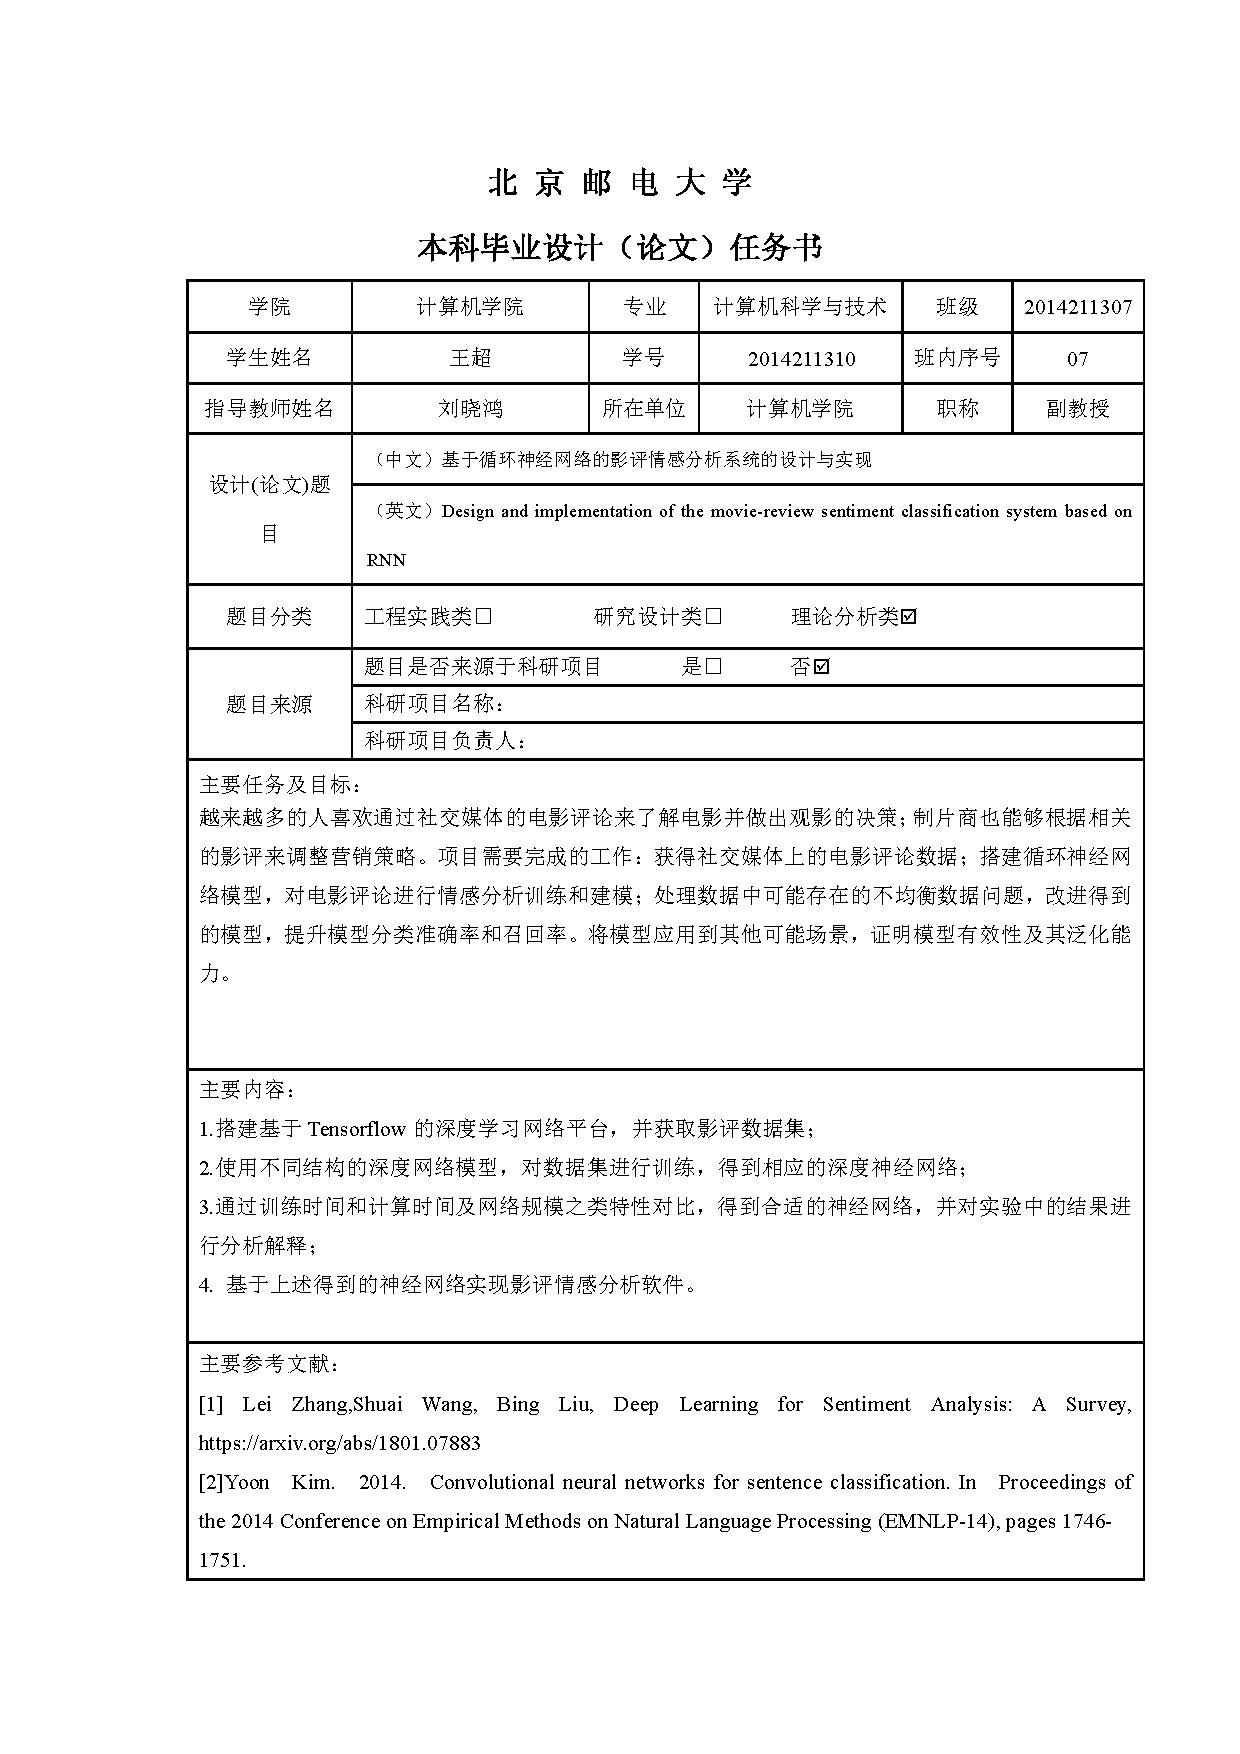
\includepdf[pages=-]{docs/task.pdf}
\newpage

% 成绩评定表
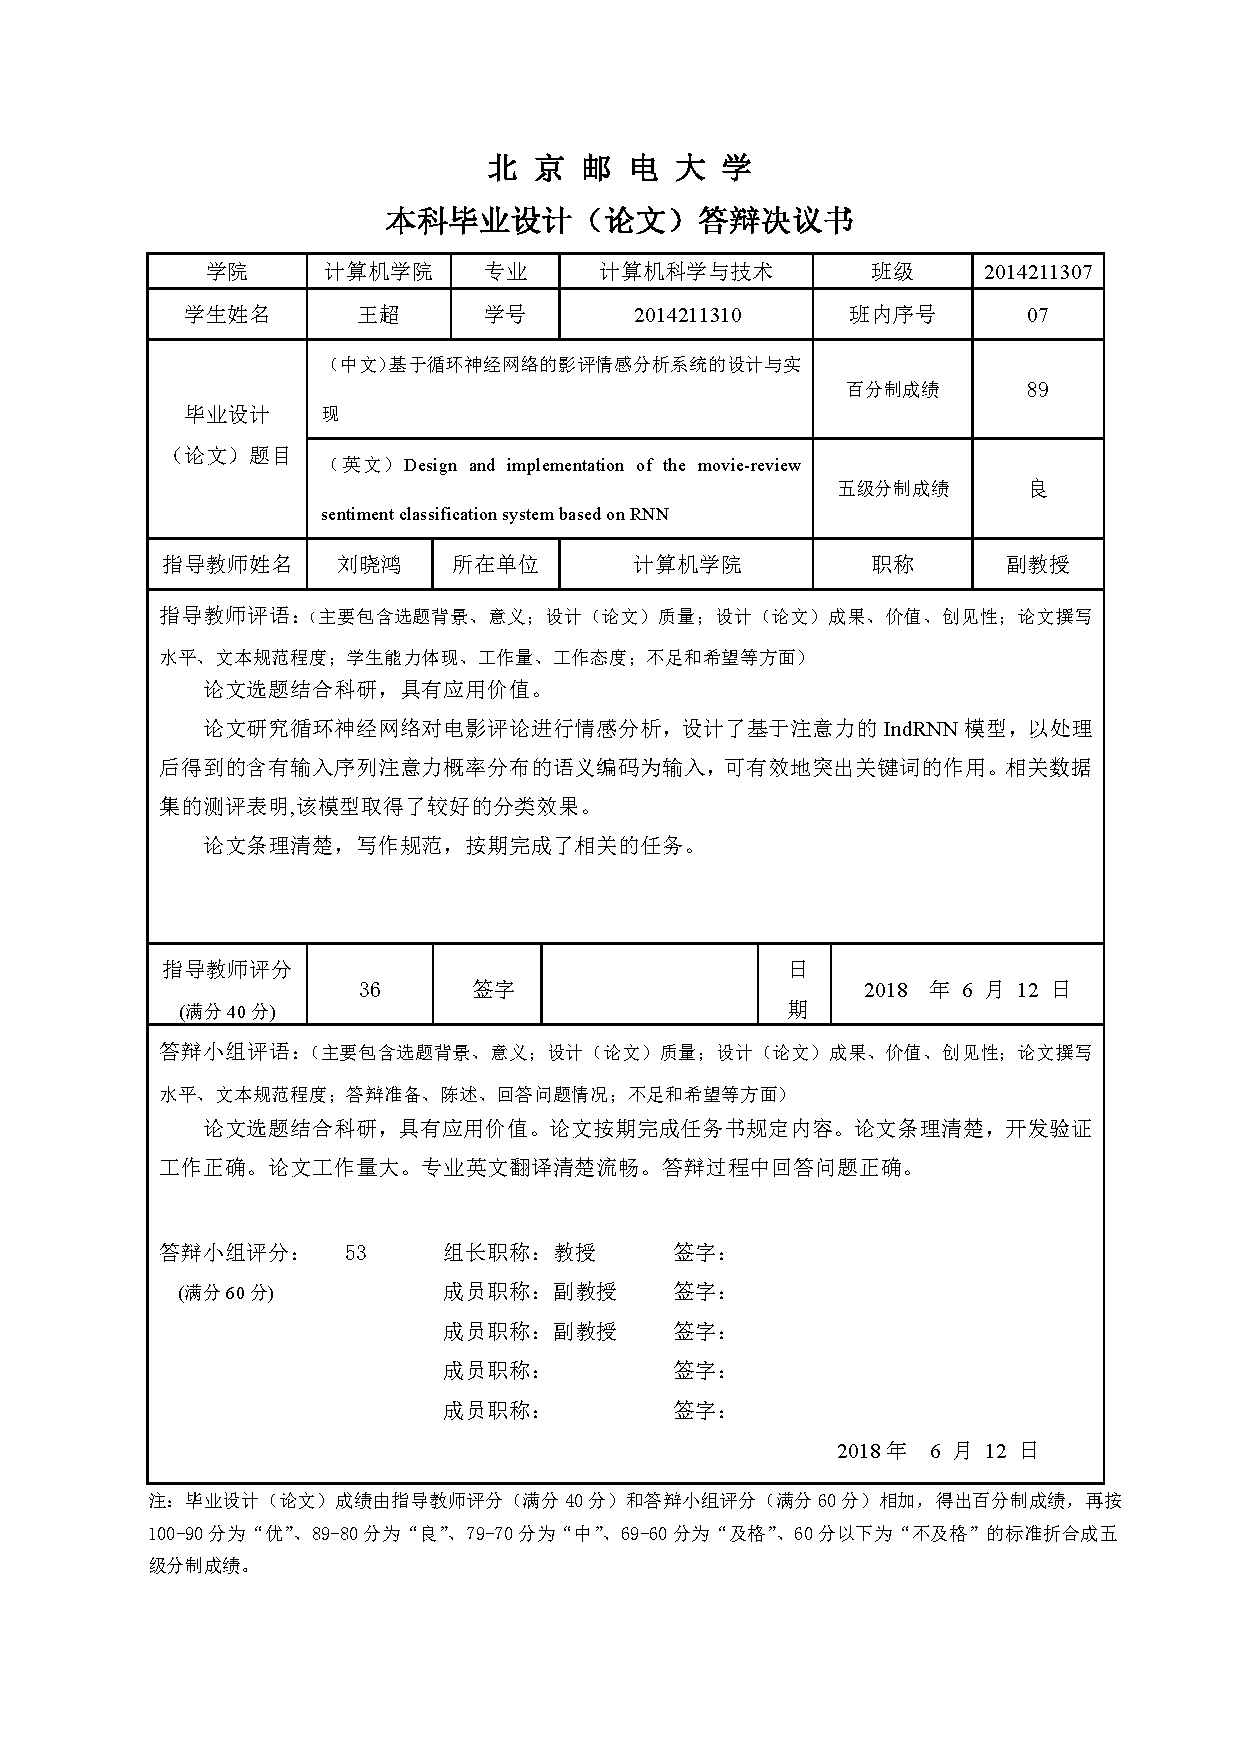
\includepdf[pages=-]{docs/scoreTable.pdf}
\newpage
\mbox{}
\thispagestyle{empty}
\newpage
% 诚信声明

\includepdf[pages=-]{docs/statement.pdf}
\newpage

% \mbox{}
% \thispagestyle{empty}
% \newpage

%%%%%%%%%%%%%%%%%%%%%%%%%%%%%%%%%%%%%%%%%%%%%%%%%%%%%%%%%%%%%%%%%%%%
%                                                                  %
%   Copyright (c) 2010 - 2011 Caspar Zhang <casparant@gmail.com>   %
%                                                                  %
%   This copyrighted material is made available to anyone wishing  %
%   to use, modify, copy, or redistribute it subject to the terms  %
%   and conditions of the GNU General Public License version 2.    %
%                                                                  %
%   This program is distributed in the hope that it will be        %
%   useful, but WITHOUT ANY WARRANTY; without even the implied     %
%   warranty of MERCHANTABILITY or FITNESS FOR A PARTICULAR        %
%   PURPOSE. See the GNU General Public License for more details.  %
%                                                                  %
%   You should have received a copy of the GNU General Public      %
%   License along with this program; if not, write to the Free     %
%   Software Foundation, Inc., 51 Franklin Street, Fifth Floor,    %
%   Boston, MA 02110-1301, USA.                                    %
%                                                                  %
%%%%%%%%%%%%%%%%%%%%%%%%%%%%%%%%%%%%%%%%%%%%%%%%%%%%%%%%%%%%%%%%%%%%

% 你只需要修改下面几行就可以完成大部分内容的填写,
% 这要求你具有一定的LaTeX基础,但是如果你足够聪明,
% 不具有LaTeX基础也可以完成。

% 论文中文题目
\def\thesistitle{基于循环神经网络的影评情感分析系统的设计与实现}

% 论文英文题目
\def\thesistitleen{Design and implementation of the movie-review sentiment classification system based on RNN}

% Thank Words
\def\thankwords{

在本篇本科学位论文完成之际,本人也将结束4年的本科生生活。在结束大学生活,走向工作岗位之际,衷心向帮助过我的老师、同学、朋友及家人表示感谢。

本论文使用基于LaTeX的本科生毕业设计模板书写,衷心感谢Caspar Zhang等人开源的这份模板。
}
    % Main items
%%%%%%%%%%%%%%%%%%%%%%%%%%%%%%%%%%%%%%%%%%%%%%%%%%%%%%%%%%%%%%%%%%%%
%                                                                  %
%   Modified by Bing Hsu <hello@antinucleon.com> 2013              %
%   Forked From (c) 2010 - 2011 Caspar Zhang <casparant@gmail.com> %
%                                                                  %
%   This copyrighted material is made available to anyone wishing  %
%   to use, modify, copy, or redistribute it subject to the terms  %
%   and conditions of the GNU General Public License version 2.    %
%                                                                  %
%   This program is distributed in the hope that it will be        %
%   useful, but WITHOUT ANY WARRANTY; without even the implied     %
%   warranty of MERCHANTABILITY or FITNESS FOR A PARTICULAR        %
%   PURPOSE. See the GNU General Public License for more details.  %
%                                                                  %
%   You should have received a copy of the GNU General Public      %
%   License along with this program; if not, write to the Free     %
%   Software Foundation, Inc., 51 Franklin Street, Fifth Floor,    %
%   Boston, MA 02110-1301, USA.                                    %
%                                                                  %
%%%%%%%%%%%%%%%%%%%%%%%%%%%%%%%%%%%%%%%%%%%%%%%%%%%%%%%%%%%%%%%%%%%%

%%%%%%%%%%%%%%%%%%%%%%%%%%%%%%%%%%%%%%%%%%%%%%%%%%%%%%%%%%%%%%%%%%%%
%                                                                  %
%   Copyright (c) 2010 - 2011 Caspar Zhang <casparant@gmail.com>   %
%                                                                  %
%   This copyrighted material is made available to anyone wishing  %
%   to use, modify, copy, or redistribute it subject to the terms  %
%   and conditions of the GNU General Public License version 2.    %
%                                                                  %
%   This program is distributed in the hope that it will be        %
%   useful, but WITHOUT ANY WARRANTY; without even the implied     %
%   warranty of MERCHANTABILITY or FITNESS FOR A PARTICULAR        %
%   PURPOSE. See the GNU General Public License for more details.  %
%                                                                  %
%   You should have received a copy of the GNU General Public      %
%   License along with this program; if not, write to the Free     %
%   Software Foundation, Inc., 51 Franklin Street, Fifth Floor,    %
%   Boston, MA 02110-1301, USA.                                    %
%                                                                  %
%%%%%%%%%%%%%%%%%%%%%%%%%%%%%%%%%%%%%%%%%%%%%%%%%%%%%%%%%%%%%%%%%%%%

% 你只需要修改下面内容就可以完成中英文摘要,
% 这要求你具有一定的LaTeX基础,但是还是那句话,
% 如果你足够聪明,不具有LaTeX基础也可以完成。

% 中文摘要
\def\abstractzh{
%从这里开始写你的摘要,分段需要空一行。
在自然语言处理领域里,情感分析已经被广泛应用,一般划分为以下几个部分:文本的预处理、文本特征的提取、机器学习分类器训练等方面。随着深层神经网络模型在图像识别,机器翻译等领域内的巨大进展,深层神经网络模型被证明在文本特征向量提取方面有着巨大的优势。

本文的研究内容是循环神经网络在情感分析领域对电影评论的研究。主要结合时下性能较好的循环神经网络方法,进行分析比较并结合。本文要基于word2vec使用模型,采用了Word Embedding机制训练包含语义特征的词向量,避免了高维度输入易产生维度灾难的问题。同时,基于Word Embedding训练出的词向量具有相似度的特征,具备了一定的语义信息,作为Attention-Based IndRNN模型的输入,对二值分类器的性能具有一定的提高效果。

在文本特征提取问题上,基于时下较为优异的模型,本文设计了Attention-Based IndRNN和Attention-Based Bi-IndRNN模型,其中IndRNN相对传统RNN和LSTM来说,解决了梯度消失和梯度爆炸的问题。同时本文通过Attention-Based的方法,得到含有输入序列注意力概率分布的语义编码,并将其作为二值分类器的输入,减少了特征向量提取过程中的信息丢失和信息冗余,可以有效地突出关键词的作用。该方法可以得到包含注意力概率分布的语义特征,并对特征提取部分进行优化。基于豆瓣影评及IMDB影评数据集进行测评,结果表明:这两个模型在多个情感分析任务中都取得了相对较好的效果。
}

% 中文关键字
% TODO: 改成可变长度的
\def\abszhkeyone{循环神经网络}
\def\abszhkeytwo{情感分析}
\def\abszhkeythree{长短时记忆}
\def\abszhkeyfour{独立循环神经网络}
\def\abszhkeyfive{注意力模型}

% ABSTRACT
\def\abstracten{
In the field of natural language processing, sentiment analysis has been widely used and is generally divided into the following sections: text preprocessing, text feature extraction, machine learning classifier training and so on. As deep learning technology has made great progress in image recognition, machine translation and other fields, the deep learning model has been proved to have great advantages in data preprocessing and feature extraction.

The research content of this paper is the research of film review in the field of sentiment analysis by cyclic neural network. Mainly combined with the current method of better performance of the circulatory neural network, analysis and comparison. This article is based on the word2vec use model, using the Word Embedding mechanism to train the word vectors containing semantic features, to avoid the problem of dimensional disaster caused by high-dimensional input. At the same time, the word vectors trained based on Word Embedding have similarity features and possess certain semantic information as input to the Attention-Based IndRNN model, and the performance of the binary classifier.

On the issue of text feature extraction, based on the current excellent model, this paper designs Attention-Based IndRNN and Attention-Based Bi-IndRNN models. IndRNN solves the problem of gradient disappearance and gradient explosion compared to traditional RNN and LSTM. At the same time, this paper adopts Attention-Based method to obtain the semantic code containing the attention probability distribution of the input sequence, and uses it as the input of the binary classifier to reduce the information loss and information redundancy in the feature vector extraction process, which can effectively Highlight the role of keywords. This method can get the semantic features containing attention probability distribution, and optimize the feature extraction part. Based on the evaluation of Douban film criticism and IMDB film review dataset, the results show that these two models have achieved relatively good results in multiple sentiment analysis tasks.
}

% Key Words
% TODO: 改成可变长度的
\def\absenkeyone{Recurrent neural network}
\def\absenkeytwo{sentiment analysis}
\def\absenkeythree{long short time memory}
\def\absenkeyfour{independent recurrent neural network}
\def\absenkeyfive{Attention model}


% 中文摘要
\begin{titlepage}
    \begin{spacing}{1.05}
        \centering
        \parbox[c]{.6\textwidth}{\thesistitlefont{\thesistitle}}
    \end{spacing}

    \begin{spacing}{1.6}
        \centering
        \sanhao\quad{} \\
        \abszhname{摘\quad{}要} \\
        \xiaosanhao\quad{}
    \end{spacing}

    \normalsize

    \abstractzh

    \quad{}

    \abszhkey{关键词}\quad{}%
    \abszhkeys{\abszhkeyone\quad{}%
                      \abszhkeytwo\quad{}%
                      \abszhkeythree\quad{}%
                      \abszhkeyfour\quad{}%
                      \abszhkeyfive}%
\end{titlepage}

\mbox{}
\thispagestyle{empty}
\newpage

% Abstract
\begin{titlepage}
    \begin{spacing}{1.05}
        \centering
        \parbox[c]{.6\textwidth}{\thesistitleenfont{\thesistitleen}}
    \end{spacing}

    \begin{spacing}{1.6}
        \centering
        \sanhao\quad{} \\
        \abszhname{ABSTRACT} \\
        \xiaosanhao\quad{}
    \end{spacing}

    \normalsize

    \abstracten

    \quad{}

    \absenkey{KEY WORDS}\quad{}%
    \absenkeys{\absenkeyone\quad{}%
                      \absenkeytwo\quad{}%
                      \absenkeythree\quad{}%
                      \absenkeyfour\quad{}%
                      \absenkeyfive}%
\end{titlepage}
%
\mbox{}
\thispagestyle{empty}
\newpage
  % Abstract
\frontmatter\tableofcontents % Content

% 正文
\newpage\mainmatter
\fancypagestyle{plain}{\pagestyle{fancy}} % Add head to new chapter
\pagestyle{fancy} % Head and foot
%\let\cleardoublepagebak=\cleardoublepage
%\let\cleardoublepage\relax % Make new chapter stay on old page

%%%%%%%%%%%%%%%%%%%%%%%%%%%%% Main Area %%%%%%%%%%%%%%%%%%%%%%%%%%%%

\chapter{绪论}
\section{研究背景及意义}
信息传播的方式经历了语言符号、文字、电子传播等演变过程。21世纪起,互联网逐渐成为人与人之间的沟通媒介。随着其发展,许多现代化的通讯交流方式建立了起来,越来越多的用户开始藉由互联网发表着自己的观点。由于这种现象,越来越多的观点和想法正在互联网上传播和发布。根据第41次《中国互联网络发展状况统计报告》,我国约有55.8\%的人已经使用了互联网。任意一项商品或服务就会产生成千上万的评价信息,这就使得用户评论成为了一种越发重要的信息载体。例如,微信朋友圈、QQ空间用户占比分别为87.3\%和64.4\%,微博作为社交媒体,使用率也达到了40.9\%。知乎、豆瓣的用户使用率也分别有14.6\%和12.8\%。从微博到豆瓣,社交网站和内容评论网站中蕴含了大量关于个人观点、评论的数据。

互联网包含海量的信息,人们可以利用它来帮助自己对特定问题做出决定。绝大多数人在决定某件事前会试图在网上找到相关产品,比如他们会考虑想去旅行的国家或考虑看的电影的评价。人们可以从这些网站中收集和分析关于特定主题的许多意见和观点。随着电子商务的发展,在电影市场的下游环节,用户可以通过在线票务系统选择影片、影院并在观影结束后进行点评,这一系列的行为所产生的大量数据,能够为电影产业的上游环节提供重要思考。在传统电影行业中是“我生产什么观众就看什么”,用户只能被动接受,可选择性小。而在互联网环境下,观众由产生观影意向到走进影院、完成观影,会经过“搜索关注、购票观看、评分评论”三个阶段,不管在哪一个阶段,用户的主体地位都已经被默许\cite{shenyaoZhongGuoDianYingZaiXianPiaoWuFaZhanYanJiu2016}。

2012年,国内学者殷国鹏等采用信息采纳理论作为研究基础,讨论了消费者在购买决策中受评论的两类影响因素,即评论特征和评论者要素,并融合社会网络视角构建了评论有用性模型\cite{yinguopengWangLuoSheQuZaiXianPingLunYouYongXingYingXiangMoXingYanJiuJiYuXinXiCaiNaYuSheHuiWangLuoShiJiao2012}。社交媒体的电影评论对于购票者做出决产生了一定的影响。制片商也能够根据相关的影评来调整营销策略。

但是,面对如此庞大的评论文本信息,传统的通过人工获取评论的情感倾向是一件特别费时费力的事情。因此,现在已经出现了对文本的情感分析过程自动化的需要。这将有助于人们能够以合理便捷的方式获得关于特定主题的意见和观点,而不是让他们搜索和阅读评论以获得最终意见。对于电影的上游,企业市场中,时间对企业来说比对普通用户更有价值,更需要一个自动化系统来帮助他们确定其产品和服务的用户的意见和看法。一个可以获取和分析用户评论以了解最终情绪的工具对企业更有价值。

情感分析已被证明对于几种自然语言处理(NLP)任务(如应答系统和信息提取)是有益的\cite{pangOpinionMiningSentiment2008}。信息提取(IE)旨在提取与特定主题或需求相关的信息。例如,现在人们倾向于使用互联网,通过使用论坛或其他社交网络来传播他们对主题或问题的想法和想法。其中一些想法是积极的,而另一些想法和内容则有些负面。

这种在线传播情感的概念在文本分析中创造了一个新的领域,将传统的以事实和信息为中心的文本观点扩展到研究主题,以启用情感感知型应用。在过去的十年中,从文本中提取情感在工业界和学术界都引起了高度关注。形式上,情感分析试图从人们的写作中提取人们的观点。这个主题包括许多领域,例如自然语言处理,机器学习和计算语言学。

目前为止,情感分析的主要方法分别为基于情感词典的情感分析方法和基于机器学习的情感分析方法。由于,基于情感词典的方法的性能相对机器学习方法来说,十分容易受到情感词典的大小与水平影响,因此本文将主要研究基于机器学习的方法来进行情感分析。

\section{国内外研究现状}

2003年,J. Yi等人提出通过提取情感特征基于情感词典的情感分析器 \cite{yiSentimentAnalyzerExtracting2003}。2007年,徐琳宏提出了根据分析句子结构提取情感特征,基于情感词典分析情感倾向\cite{xulinhongJiYuYuYiZiYuanDeWenBenQingGanJiSuan2007}。基于规则、情感词典的情感分析方法长期有学者在研究,不过随着Pang等人提出了基于机器学习的方法如朴素贝叶斯(Naive Bayes)、最大熵分类(Max Entropy)和支持向量机(SVM)等来对文本通过整体情感进行正负面分类\cite{pangThumbsSentimentClassification2002}。由于基于情感词典的分析方法的进步空间相对机器学习方法更易受到语料库限制,在这之后,基于机器学习方法的情感分类模型被越来越多的学者研究。在这个过程中学者们发现,从文本中提取的特征被严重依赖,传统统计方法如N-gram模型存在维度灾难问题。根据Bengio等人在2003年的研究,神经网络能够有效解决维度灾难问题,初步使用到了词向量\cite{bengioNeuralProbabilisticLanguage2003}。在2010年,Mikolov等人提出了基于循环神经网络的语言模型来提高神经网络语言模型的性能,同样使用到了词向量\cite{mikolovRecurrentNeuralNetwork}。在2013年,Mikolov等人使用CBOW和Skip-Gram模型训练了具有语义特征的词向量\cite{mikolovEfficientEstimationWord2013}。之后,他们提出了基于Skip-Gram模型的改进,提出了词向量蕴含大量语法、语义的观点\cite{mikolovDistributedRepresentationsWords2013a}。2014年,Quoc等人进行了词向量与BOW等模型的比较,发现其性能的优异性\cite{leDistributedRepresentationsSentences}。Mikolov等人后来发布了开源模型Word2vec,本文中使用的词向量就是word2vec训练得到的。

国外,2013年,Vivek等人研究了提高朴素贝叶斯在分类方面的性能的一些方法\cite{narayananFastAccurateSentiment2013}。2014年,Kim提出了使用卷积神经网络训练模型进行情感分类,性能较佳\cite{kimConvolutionalNeuralNetworks2014a}。2012年,Socher提出了Matrix-Vector RNN模型进行情感分类\cite{socherSemanticCompositionalityRecursive}。2013年,Socher对影评使用RNTN(Recursive Neural Tensor Network)进行情感分类,相对传统SVN、Matrix-Vector RNN等方法取得了较好的结果\cite{socherRecursiveDeepModels2013}。2014年,dos Santos提出一个新的深度卷积神经网络(CharsSCNN)对短文本进行情感分类取得了较好高的准确度\cite{dossantosDeepConvolutionalNeural2014}。Irsoy等人提出了一个深度递归神经网络进行情感分析,性能相比以往RNTN等较为优异\cite{irsoyDeepRecursiveNeural2014}。Chung等人对LSTM、GRU模型进行了一些改进\cite{chungEmpiricalEvaluationGated2014}。2015年,Kai将LSTM推广到树状网络拓扑结构(Tree-LSTM)进行情感分析\cite{taiImprovedSemanticRepresentations2015}。2016年,Lee提出了一个基于递归神经网络和卷积神经网络的模型进行短文本序列分类\cite{leeSequentialShortTextClassification2016}。Ghosh等人将LSTM与传统机器学习方法相结合,有效提高了情感分类模型的性能\cite{ghoshDocumentModelingHierarchical2018}。

国内方面,2014年,Tang等人学习了SSWE(sentiment-specfic 词向量)模型用于twitter情感分类中\cite{tangLearningSentimentSpecificWord2014}。Li等人提出了自适应递归神经网络对twitter进行情感分类\cite{dongAdaptiveRecursiveNeural2014}。朱少杰提出了融合深度学习特征的半监督RAE方法进行情感分类\cite{zhushaojieJiYuShenDuXueXiDeWenBenQingGanFenLeiYanJiu2014}。2015年,Tang等人引入神经网络模型(ConvGRNN和LSTM-GRNN)用于文档级别的情感分类\cite{tangDocumentModelingGated2015}。梁军等人提出了基于极性转移和LSTM递归神经网络的情感分析\cite{liangjunJiYuJiXingZhuanYiHeLSTMDiGuiWangLuoDeQingGanFenXi2015}。2016年,刘艳梅提出了基于SVM/RNN的情感分类器\cite{liuyanmeiShenDuXueXiJiZhuXiaDeZhongWenWeiBoQingGanDeFenXiYuYanJiu2016}。2017年,李丹将LSTM模型、NBSVM模型以及doc2vec模型相融合进行了情感分析\cite{lidanJiYuChangDuanShiJiYiWangLuoDeZhongWenWenBenQingGanFenXi2017}。李松如改进了RNN-Attention模型,取得了较好的性能\cite{lisongruJiYuXunHuanShenJingWangLuoDeWangLuoYuQingWenBenQingGanFenXiJiZhuYanJiu2017}。成璐提出了基于注意力机制的双向LSTM模型的情感分类应用\cite{chengluJiYuZhuYiLiJiZhiDeShuangXiangLSTMMoXingZaiZhongWenShangPinPingLunQingGanFenLeiZhongDeYanJiu2017}。2018年,李松如等人提出了基于循环神经网络的情感词注意力模型进行情感分析,相比传统模型,性能有所提升\cite{lisongruCaiYongXunHuanShenJingWangLuoDeQingGanFenXiZhuYiLiMoXing2018}。


\section{研究内容介绍}

本文的主要研究内容和研究成果总结如下:
(1)本文的研究内容是循环神经网络在情感分析领域对电影评论的研究。主要结合时下性能较好的循环神经网络方法,进行分析比较并结合。本文要基于word2vec使用模型,采用了词向量机制训练包含语义特征的词向量,避免了高维度输入易产生维度灾难的问题。同时,基于词向量训练出的词向量具有相似度的特征,具备了一定的语义信息,作为Attention-Based IndRNN模型的输入,对二值分类器的性能具有一定的提高效果。
(2)在文本语义提取问题上,基于时下较为优异的模型,本文设计了Attention-Based IndRNN模型和Attention-Based Bi-IndRNN模型,其中IndRNN相对传统RNN和LSTM来说,解决了梯度消失和梯度爆炸的问题。同时本文通过Attention-Based的方法,得到含有输入序列节点注意力概率分布的语义编码,并将其作为分类器的输入,减少了特征向量提取过程中的信息丢失和信息冗余,令关键词的作用凸显了出来。该方法可以得到包含注意力概率分布的语义特征,并对特征提取部分进行优化。


\section{文本的组织结构}
本文一共分为五个章节,主要内容如下所示:

第一章为绪论部分,该章主要介绍有关本文课题的研究背景及意义,在情感分析领域中的国内外研究现状,以及本文对中文文本情感分析主要采用的方法。

第二章为情感分析的相关技术介绍,主要介绍了本文的课题研究中需要了解到的一些基础知识,算法和一些具体的应用。主要包括了中文分词技术的介绍,以及在文本情感分析研究中的一些深度学习算法的极少。

第三章为词向量表示部分,主要介绍了词向量表示技术以及本文主要使用的神经网络预测模型。

第四章为本文的重点部分,详细地介绍了本文研究课题所采用的中文文本情感分析算法Attention-Based IndRNN对中文文本情感分析的具体过程。其中包括了使用IndRNN对中文文本进行情感分析的原因,传统的循环神经网络的不足之处。

第五章为对比实验部分,介绍了在收集的评论数据集上,例如豆瓣的电影评论和IMDB评论数据集,进行对比实验得到的结果,并针对该结果做一些分析。

第六章为本文的总结与展望部分,主要讲述了本文在实验中遇到的一些问题和进一步需要改进的方向。


\chapter{情感分析的相关技术综述}
文本情感分析是时下比较常见的应用。本章将介绍情感分析主要运用到的一些相关技术。

情感分析的一般流程图如下:

\buptfigure[width=0.7\textwidth]{pictures/structure.png}{情感分析流程图}{structure}

纵观中英文文本的情感分析的预处理过程,英文具有一种天然的分词结构,以空格为界可以很清晰的区分词义。而中文,天然以语句为单位,划分词义并不能直接从语句中得到。所以,相比英文的处理,中文文本在自然语言处理的过程中首先需要进行中文分词。出于后续情感分析模型的训练中,语义的提取对词义的表示十分重视,因而中文分词的好坏对后续训练具有极大的影响。所以,在本章节中,将介绍中文文本的一些分词技术,为之后的情感分析打下一个好的基础。

主要有两种类型的情感分析方法,一类是基于情感词典的分析方法,一类是转化为文本分类问题来处理。

本文将中文文本情感分析转化为中文文本情感二值分类问题,之后得到情感倾向判断。


\section{中文分词}
对于英文语句而言,空格是天然的分隔符,单词之间非常自然的分词结构。而对于中文语句来说,词与词之间不存在这样的分隔符,只有能够比较明显的分隔的字、句、段。在中文文本中,有很多需要用多个字来表达情感的词与,无法直接分隔字来进行获取情感词。所以,首先需要对中文文本进行分词,从而才能用于训练模型。中文分词,是指将词按顺序逐个拆分,将一个完成连续的序列拆分成多个序列组合的过程。

中文分词技术主要有以下三类,基于词表的分词方法、基于统计语言模型的分词方法和基于序列标注的分词方法。

基于词表的分词方法主要由正向最大匹配法(forward maximum matching method, FMM)和逆向最大匹配法(backward maximum matching method, BMM)等组成。这种类型的技术也被称为字符串匹配分词算法。这个方法主要是将待匹配字符串按照某些策略与词表进行匹配,匹配到了就取出来。这种方法有效率高的优点,但对于歧义词、网络上的新词无法进行很好的划分。
基于统计语言模型的分词方法主要有基于N-gram语言模型的分词方法。文本序列的划分存在多种结果,N-gram模型是利用统计语言模型找出其中概率最大的一条。这种方法对于歧义词与网络新词的划分能得到比较好的结果。

基于序列标注的分词方法主要有基于隐马尔科夫模型(Hidden Markov Model, HMM)的分词方法、基于最大熵马尔科夫模型(Maximum Entropy Markov Model, MEMM)的分词方法、基于条件随机场(Conditional Random Field, CRF)模型的分词方法等。这类方法的基本思路是对汉字进行标注训练,结合词语出现频率与上下文,具有一定的学习能力。因此对歧义词与网络新词同样具有非常好的结果。

上述这些分词方法都有各自的优点,但也存在缺点。现在常用的分词器都是综合多种方法,使用机器学习方法与词典相结合进行分词。如Jieba分词器的词图扫描主要是藉由前缀词典来实现,生成一个包含句子中所有可能词组合而形成的的有向无环图(DAG),其最大概率路径主要使用动态规划算法来寻找,最后基于词频找出最佳划分组合。面对分词比较常见的新词问题,主要通过隐马尔科夫(Hidden Markov Model,HMM)模型,该模型由维特比算法(Viterbi)实现。该分词器由于性能优异,本文使用Jieba分词器来对文本进行分词处理。

\section{使用机器学习算法的情感分析}

在情感分析问题中,最重要的部分是通过某种机器学习算法来实现模型的训练和预测结果。一般是将情感分析作为分类问题,例如二值分类等等来处理。

分类问题,可以划分为三类方法,基于规则的分类模型、基于机器学习的分类模型和基于神经网络的方法。基于规则,可以使用例如决策树(Decision Tree)、随机森林(Random Forest)、RIPPER算法等。基于机器学习,可以使用线性分类器(逻辑回归),支持向量机(Support Vector Machine, SVM)或者朴素贝叶斯分类器(Naive bayes classfier, NB)来处理。基于神经网络的方法,一般使用多层感知机(Multiayer Perceptron, MLP), 卷积神经网络(Convolutional Neural Network, CNN)和循环神经网络(Recurrent Neural Network, RNN)等。

根据国内外现状,基于神经网络的方法在性能上较佳,因而本文主要采用了循环神经网络来进行训练。

\subsection{RNN模型}
循环神经网络(Recurrent Neural Networks, RNN)是计算图包含有向周期的人工神经网络。与前馈神经网络不同,前向神经网络中信息严格按照层与层之间的一个方向流动,在循环神经网络(RNN)中,信息按照层与层之间的循环传播,以便模型的状态根据先前状态值的变化而变动。尽管前馈神经网络可以被认为是无状态的,但是RNN具有允许模型记忆关于其过去计算的信息的记忆器。这使得循环神经网络能够表现为动态时间行为和输入-输出对的模型序列。

因为它们可以构建出输入-输出对的时间序列模型,所以循环神经网络能够将信息持久化,能够提取序列数据中的特征,对于处理具有时间性的序列数据具有相当好的效果。详细地来说,RNN会对过去的信息进行记忆并输入到当前单元的计算中,即隐藏层的输入包含上一时刻隐藏层的输出以及输入层的输出。以下是典型的RNN:

\buptfigure[width=0.7\textwidth]{pictures/RNN_1.jpg}{循环神经网络及其计算涉及的计算时间的展开}{RNN_1}

上图显示了一个正在展开(或展开)为完整网络的RNN。通过展开,我们可以看到完整序列的网络。例如,如果我们关心的序列是5个单词的句子,则网络将展开成5层神经网络,每个单词一层。管理在RNN中发生的计算的公式如下:

首先,当前时间的输入由上一时间即t-1时间的隐藏层和当前时间即t时间的输入层一起计算而得。公式如下:
$$ x(t)=w(t)+s(t-1) $$
其次,前面t-1时间内的所有词向量的时序信息都会被t-1时间的隐藏层记录下来,t时间会读入当前时间的词向量$w(t)$和t-1时间的隐藏层$s(t-1)$,和转移矩阵U和W进行矩阵乘法,最后映射到t时间的隐藏层s(t)。隐藏层的计算公式如下:
$$ s_j{(t)}=f(\sum_t{w_i{(t)} \times u_{ji}} + \sum_j{s_i{(t-1)}*w_{ji}}) $$
上式中,$ f(z) $是隐藏层的激活函数。

最后,上述结果被传入输出层。输出层的大小与词表相同,词表中第i个词汇在语句中出现的概率由第i个节点输出的值表示。输出层计算公式如下:
$$ y_k{(t)}=g(\sum_j{s_j{(t)} \times v_{kj}}) $$
上式中,$g(z)$为输出层的激活函数。


\buptfigure[width=0.7\textwidth]{pictures/RNN_basic_cell.png}{一个简单的循环神经网络}{RNN_basic_cell}

从上述循环神经网络的流程中,可以很清楚的看到可以优化的参数: 输入的词向量$x(t)$, 隐藏层的向量$s(t)$,以及共享的转移矩阵$W$, $U$和$V$。

RNN模型的训练过程和传统神经网络模型训练过程是类似的,有一些基础名词需要了解。

% \subsubsection{损失函数和激活函数}
% 由于其优美的派生形式,sigmoid函数(也称为逻辑函数)经常用作激活函数。
% $$ y = f(z)=\frac{1}{1+e^{-x}} $$
% $$ f\prime(z) = y(1-y) $$
% 事实上,对于指数族概率分布(例如softmax)的任何概率函数,
% $$ g(z)=\frac{e^x}{\sum_k{e^z_k}} $$
% 激活函数求导都是成立的。
%
% 当然,这不是使sigmoid函数如此具有吸引力的唯一原因。它肯定有其他一些好的属性。但据我所知,这是最令人吃惊的一个。
%
% 损失函数可以是任何不同的函数,它能够测量黄金答案中预测值的损失。SSE损失函数经常使用,并且在传统的前馈神经网络的训练中运行良好。
%
% 对于循环神经网络,另一个适当的损失函数是所谓的交叉熵:
%
% 交叉熵损失用于循环神经网络语言模型并且性能良好。以sigmoid或softmax作为激活函数,交叉熵损失具有良好的性质:


% 然后,误差(向量)递归地向后传播然后,相应地更新输入权重V和递归权重U.

% \paragraph{梯度下降算法}
%
% 训练神经网络的目的是最小化损失函数的权重和偏置,现在主要有梯度下降方法和Adam方法等。
%
% 梯度下降(Gradient Descent)法,每次通过以下公式来更新权重:
% $$ W_k \prime = W_k - \eta \frac{\partial{C}}{\partial{W_k}} $$
% $$ b_l \prime = b_l - \eta \frac{\partial{C}}{\partial{b_l}} $$
%
% 其中,$\eta$为学习率,$C$是定义的损失函数,输出为我们使用当前的权重计算出的输出。
%
% \paragraph{反向传播算法}
% 任何前馈神经网络都可以使用反向传播(BP)算法进行训练,只要损失函数是可以忽略的。BP实际上是一个传播梯度下降算法,其中梯度向后传播,导致非常高效地计算更高层的权重变化。根据梯度下降,相对于特定的权重,网络中的每个权重变化应该与损失函数的负梯度成比例。
%
% 反向传播训练算法的目标是修改神经网络的权重,以便与响应于相应输入的一些预期输出相比网络输出的误差最小化。这是一种监督学习算法,可以根据所做出的具体错误纠正网络。一般算法如下:
%
% 反向传播算法核心解决的问题是针对损失函数C计算$\frac{\partial C}{\partial w}$和$\frac{\partial C}{\partial b}$
%
% 为了计算这两个,引入中间变量$\delta_{j}^{l}$,表示第l层第j个神经元的误差。
%
% $\delta_{j}^{l}$的定义是:
% $$ \delta _{j}^{l}=\frac{\partial C}{\partial z_{j}^{l}} $$
%
% 损失函数$C$可以看作是关于$z$的函数,而$z$是$W$和$b$的线性组合。
%
% \begin{algorithm}
% \floatname{algorithm}{算法}
% \caption{反向传播算法(BP)}
% \label{algorithm_BP}
% \begin{algorithmic}[1]
% \State 输入x: 为输入层设置对应的激活值$a^1$ ,训练并通过网络传播以获得输出。
% \State 前向传播: 对每个$l=2,3,\dots ,L $计算相应的$z^l=w^l a^{l-1} + b^l$和$a^l = \sigma(z^l)$
% \State 输出层误差$\delta^L$: 计算向量$\delta^{L}=\nabla_a C \odot \sigma'(z^L)$
% \State 反向传播误差: 对每个$l=L-1, L-2, \dots, 2$, 计算$ \delta^L=((w^{l+1})^T\delta^{l+1}) \odot \sigma'(z^l) $
% \State 输出: 损失函数的梯度由$\frac{\partial C}{\partial w_{jk}^{l}}=a_{k}^{l-1}\delta_{j}^{l} $和$ \frac{\partial C}{\partial b_j^{l}}=\delta_j^l$得出
% \end{algorithmic}
% \end{algorithm}
%
% BP的4个基本公式可以用于计算$\delta^{l}$和损失函数的梯度:
% \paragraph{输出层误差$\delta^{L}$的计算公式}
% $$ \delta_{j}^{L}=\frac{\partial C}{\partial z_{j}^{L}}=\frac{\partial C}{\partial a_{j}^{L}}\sigma'(z_{j}^{L}) $$
%
% 转换为矩阵运算,如下:
% $$\delta^{L}=\nabla_a C \odot \sigma'(z^L) \label{BP1}$$
%
% 其中,$\odot$表示elementwise运算,而$\nabla_a C$是由$\partial C / \partial a_{j}^{L}$组成的向量。
%
% \paragraph{$\delta^L$和$\delta^{L+1}$的计算公式}
%
% $$ \delta^L=((w^{l+1})^T\delta^{l+1}) \odot \sigma'(z^l) \label{BP2}$$
%
% \eqref{BP1}可以用于计算出$\delta^L$的值,而\eqref{BP2}可以根据最后一层的误差,逐步向前传递计算前面输出层的$\delta^L$值
%
% \paragraph{bias的导数计算公式}
%
% $$ \frac{\partial C}{\partial b_j^{l}}=\delta_j^l \label{BP3} $$
%
% 这个公式表明,第$l$层偏差bias的导数和第$l$层的误差值相等。
%
% \paragraph{权重$W$的导数计算公式}
% $$ \frac{\partial C}{\partial w_{jk}^{l}}=a_{k}^{l-1}\delta_{j}^{l} $$
%
% 同理,这个公式揭露出权重 W 的导数和误差以及网络输出之间的关系。用一种更简洁的方式表示为:
% $$\frac{\partial C}{\partial w} = a_{in}\delta_{out} \label{BP4} $$
%
% 其中,$a_{in}$是权重$W$的输入,而$\delta_{out}$是权重$W$对应的$z$的误差。用一幅图表示如下:
%
% %width=0.7\textwidth
% \buptfigure[]{pictures/bp_1.png}{权重的导数计算}{bp_1}
%
% 当 $a_{in} \approx 0$ 时,梯度公式的值会很小,换句话说,当权重 W 的输入 $a_{in} $,也就是上一层激活层的输出接近 0 时,那么这个激活层对网络的影响就变得很小,$W$ 的学习也会变得很慢。
%
% 反向传播训练算法适用于训练固定大小的输入-输出对上的前馈神经网络,但是序列数据按照时间顺序排序的数据就需要一定的修改了。
%
% \paragraph{随时间反向传播算法}
% 由于RNN是一种基于时序数据的神经网络模型,在RNN中,横向展开的每一层都是共享权重的,每一个输出的梯度(gradient)不仅仅依赖于当下这个时间点,还依赖于过去的时间点,因此传统的BP算法并不适用于该模型的优化,这要求我们提出新的优化算法。RNN中最常用的优化算法是随时间反向传播算法(BackPropagation Through Time,BPTT)。


% \buptfigure[width=0.7\textwidth]{pictures/RNN_unfolding.png}{一个展开的循环神经网络}{RNN_unfolding}
%
% 在循环神经网络中,错误可以进一步传播,即超过2层,以便捕获更长的历史信息。这个过程通常称为展开。展开的RNN如上图所示。
%
% 在展开的RNN中,权重在空间上以任意数量的时间步长复制。错误由于公式向后传播,递归地计算高层权重的误差增量。在获得所有错误增量之后,权重被折回,每个展开的权重增加一个大的变化。
%
% 训练循环神经网络的BPTT比通用优化技术(如演化优化)要快得多。BPTT在局部最优方面存在困难。使用递归神经网络,与前馈神经网络相比,局部最优解是一个更为重要的问题。这种网络中的循环反馈倾向于在误差表面产生混乱的响应,这会导致局部最优频繁发生,并且在误差表面上的不良位置。
%
% 循环神经网络每个时间步都显示一个输入并预测一个输出。
%
% 从概念上讲,BPTT通过展开所有输入时间步骤来工作。每个时间步有一个输入时间步,一个网络副本和一个输出。然后为每个时步计算并累计错误。网络回滚并且权重被更新。
%
% 在空间上,展开的递归神经网络的每个时间步可以被看作是附加层,给定了问题的顺序依赖性,并且来自先前时间步的内部状态被视为后续时间步的输入。
%
% BPTT的主要目的是求出$\frac{\partial C}{\partial U}$和$\frac{\partial C}{\partial W}$和$\frac{\partial C}{\partial V}$
%
% 我们可以将算法总结如下:
%
% \begin{algorithm}
% \floatname{algorithm}{算法}
% \caption{随时间反向传播算法(BPTT)}
% \label{algorithm_BPTT}
% \begin{algorithmic}[1]
% \While{True}
% \State 向网络呈现一系列输入和输出对的时间步长。
% \State 展开网络,然后计算并累积每个时间步长的误差。
% \State 汇总网络并更新权重。
% \EndWhile
% \end{algorithmic}
% \end{algorithm}
%
% 随着时间步数的增加,BPTT的计算量可能会很大。如果输入序列由数千个时步组成,那么这将是单个更新权重更新所需的衍生数量。这可能会导致权重消失或爆炸(归零或溢出),并导致慢速学习和模型技巧嘈杂。
%
% 展开的递归神经网络可以看作是一个深层神经网络,除了权重是相关的。因此,在BPTT训练中,为了保持权重的一致性,应将每个层的权重变化累加到一个较大的变化中。

% 有一种相近的算法是叫做BackPropagation Through Time(BPTS)算法,它用于训练循环神经网络[1]。实际上,在特定任务中,递归权重也可以解开。在那种情况下,要学习更多的参数。

\subsection{LSTM模型}
RNN能够运用历史信息来帮助当前的决策,但是也是存在局限性的。在实际实验中,训练模型时梯度会随着反向传播过程逐渐消失,只保持了较短范围内的序列信息。在某些需要较长的时间的信息来辅助角色时,RNN的性能就显得有所不足了,在这样的背景下,长短时记忆模型(Long Short Term Memory, LSTM)诞生了,引入了门(Gate)电路。

LSTM通过输入门、遗忘门、输出门结构来控制循环神经网络中的各个时刻的状态。这里所说的三种门实际上是sigmoid神经网络和一个按位做乘法的操作,形象的来说,sigmoid激活函数的全连接神经网络会输出0到1之间的数值,表示这个结构保留下来的信息。

LSTM的隐藏层计算输出公式如下:
\begin{equation}
    \begin{aligned}
        i_{t} & =\sigma\big(x_{t}U^{i}+h_{t-1}W^{i}\big) \\
        f_{t} & =\sigma\big(x_{t}U^{f}+h_{t-1}W^{f}\big) \\
        o_{t} & =\sigma\big(x_{t}U^{o}+h_{t-1}W^{o}\big) \\
        \tilde{C}_{t} & =\tanh\big(x_{t}U^{g}+h_{t-1}W^{g}\big) \\
        C_{t} & =\sigma\big(f_{t}\ast C_{t-1}+i_{t}\ast\tilde{C}_{t}\big)\\
        h_{t} & =\tanh(C_{t})\ast o_{t}
    \end{aligned}
\end{equation}


这里,$i, f, o$分别被称为输入,忘记和输出门。请注意,它们具有完全相同的方程,只是具有不同的参数矩阵(W,是前一个隐藏层和当前隐藏层的循环连接,U是将输入连接到当前隐藏层的权重矩阵)。他们关心所谓的门,因为sigmoid函数压缩这些向量在0和1之间的值,并且通过将它们与另一个向量相乘来确定“通过”的其他向量的数量。输入门定义了您想要通过的当前输入的新计算状态的多少。忘记门定义了你想要通过的前一个状态的多少。最后,输出门定义了你想暴露给外部网络的多少内部状态(更高层次和下一个时间步骤)。所有的门都有相同的尺寸$d_h$,你的隐藏层状态的大小。

$\tilde{C}$是基于当前输入和先前隐藏状态计算的“候选”隐藏状态。$C$是单位的内部记忆。它是前一个记忆乘以忘记门和新计算的隐藏状态乘以输入门的组合。因此,直观地说,它是我们想要如何组合先前的记忆和新的输入的组合。我们可以选择完全忽略旧的记忆(忘记全部0的门)或完全忽略新计算的状态(输入门全部为0),但很可能我们需要在这两个极端之间进行一些操作。
$h_t$是输出隐藏状态,通过将记忆器与输出门相乘来计算。并非所有内部记忆器都可能与网络中其他设备使用的隐藏状态有关。

直觉上,简单的RNN可以被认为是LSTM的特例。如果将输入门全部固定为1,将所有0的忘记门(比如说,总是忘记以前的记忆)并将输出门设置为全1(即暴露整个记忆),那么它基本就会获得传统的RNN。


\subsection{Bi-RNN模型}
单向的RNN结构能够通过前面时刻的输入来预测下一刻的输出,但也会有一些情况,预测的结果是由前面的输入与后面时刻的输入共同决定的。鉴于在这样的情况下,单向RNN的结构存在一些不足,所以提出了双向循环神经网络。单向RNN联系的是历史数据,那么双向RNN就成功联系了历史与未来。

从下图可以看到,双向RNN根据时间展开的结构,向前层和向后层共2个权值,即向前层和向后层的隐藏层与隐藏层之间的权值、向前层和向后层的隐藏层与输出层之间的权值,向前层和向后层一同连接输出层。

该模型的训练过程如下
\begin{itemize}
    \item 前向传播
    \begin{enumerate}
        \item 沿着时刻1到时刻T正向计算一遍,获取并保存每个时刻向前隐藏层的输出。
        \item 沿上述时间,反向计算一遍,获取并保存每个时刻向后隐藏层的输出。
        \item 正向和反向都计算完所有输入后,将根据每个时刻向前向后隐藏层获得最终输出。
    \end{enumerate}
    \item 反向传播
    \begin{enumerate}
        \item 计算所有时刻输出层的$\delta$项。
        \item 根据所有输出层的$\delta$项,使用 BPTT 算法更新向前层。
        \item 根据所有输出层的$\delta$项,使用 BPTT 算法更新向后层。
    \end{enumerate}
\end{itemize}

\subsection{GRU模型}
门控循环单元(Gated Recurrent Unit, GRU)背后的原理与LSTM相类似,即用门控电路机制控制输入、记忆等信息从而实现预测,它具有许多相同的属性,它将遗忘和输入门组合成一个“更新门”(Update Gate)。它还会合并单元格状态和隐藏状态,并进行一些其他更改。由此产生的模型比标准LSTM模型更简单,但其性能与序列建模的LSTM相当,但参数更少且更易于训练\cite{chungEmpiricalEvaluationGated2014}。

\buptfigure[width=0.7\textwidth]{pictures/lstm_gru.png}{GRU和LSTM}{lstm_gru}

4个公式如下:

在时间t,我们首先使用下述公式计算更新门$z_t$
$$ z = \sigma(x_t{U^2}+s_{t-1}W^{z}) $$
其中$x_t$是第t个时间的输入向量,也就是,输入序列X的第t个分量,通过线性变换(乘以权重矩阵 $W(z)$)。$h_{t-1}$ 保存前一个时间步t-1的信息,它同样也经过线性变换。更新门将这两条信息添加到Sigmoid激活函数中,并将激活结果压缩到[0,1]之间。

更新门帮助模型确定到底要将过去多少的信息传递给未来,或者需要传递前一时间步和当前时间步的信息。因为模型能决定复制过去的所有的信息以减少梯度消失的风险。

而复位门(Reset Gate)决定了过去的信息需要遗忘多少,公式见下:
$$ r = \sigma(x_t{U^r}+s_{t-1}W^r) $$

该表达式与更新门的表达式相同,只是线性变换的参数和用处不同。

如前面更新门所述,$h_{t-1}$和$x_t$先经过一个线性变换,再相加投入Sigmoid激活函数以输出激活值。

在复位门的使用中,新的记忆内容将使用复位门储存过去相关的信息,表达式见下:
$$ h = tanh(x_t{U^h}+(s_{t-1} \circ r)W^h )) $$

输入$x_t$与上一时间步$h_{t-1}$先经过一个线性变换,即分别右乘矩阵W和U.

计算复位门$r_t$与$Uh_{t-1}$的Hadamard乘积,即$r_t$与$Uh_{t-1}$的对应元素乘积。由于之前计算的复位门是0到1的向量,它会控制门控大小。例如,如果某个元素的门控值为0,那么它所包含的信息就完全被遗忘了。该Hadamard乘积将确定之前需要保留与遗忘的信息。两部分结果的和输入到双曲正切激活函数中。

在最后一步,网络需要计算$h_t$,该向量将保留当前单元的信息并传递给下一个单元。在这个过程中,我们需要使用更新门,它决定了当前记忆内容$h_t^{\prime}$和前一时间步$h_{t-1}$中需要收集的哪些信息。这一过程可以表示为:

$$ s_t = (1-z) \circ h + z \circ s_{t-1} $$

GRU有两个门,一个复位门(reset gate)和一个更新门(update gate)。直观地说,复位门会决定新输入如何与前面的记忆相合并,更新门定义了前面记忆保存到当前时间步的度量。如果我们将复位门设置为1,更新门设置为0,那样就会得到一个传统的RNN模型。

使用门控机制学习长期依赖关系的基本思路是和LSTM相似的,但仍然还存在一些关键的区别:
\begin{itemize}
    \item 将输入门、遗忘门和输出门改变为两个门:更新门和复位门。
    \item 将单元状态$c_t$与输出合并为一个状态:$h$。
    \item LSTM中的输入与遗忘门对应GRU的更新门,复位门直接作用于前面的隐藏状态。
\end{itemize}




\section{本章小结}

本章介绍了循环神经网络使用到的几个主要算法的原理及公式,梯度下降、随时间反向传播算法等。并介绍了循环神经网络的几个变体,LSTM模型、结合了LSTM单元后的双向RNN即Bi-LSTM模型、GRU模型。LSTM相比传统的RNN模型优化了长期依赖问题,可以应对长度500-1000的文本。Bi-LSTM在LSTM的基础上,保留了上下文信息。GRU模型相比LSTM模型,结构上有所简化,运行时间上有所加速。

\chapter{词向量技术}

词向量技术是将文本转换为数学方式表达的一种模型。事实证明,许多机器学习算法和几乎所有深度学习体系结构都不能以原始形式处理字符串或纯文本。他们需要数字作为输入来执行任何类型的工作,无论是分类,回归等。在文本格式中存在大量数据的情况下,必须从中提取知识并构建应用。

文本表示主要分为基于独热(one-hot Representation)的表示方法与分布式表示(Distributed Representation)的表示方法。

词向量通常会将使用字典的单词映射到矢量,如“其/表现力/还算/不错”。如独热编码向量,其中1表示该单词存在的位置并且0代表其他地方。根据上述字典以这种格式,“不错”的矢量表示是[0,0,0,1],而“表现力”的是[0,1,0,0]。

分布式表示方法现在主要分为基于矩阵(Frequecny based Embedding)的表示与基于神经网络(即Prediction based Embedding)的表示方法,词向量就属于基于神经网络的表示方法。另外,可以从上文的例子中看到,独热编码存在维度过大的问题,而词向量是将其压缩嵌入过后得到的,因而词向量也叫做词嵌入(Word Embedding)。

基于矩阵的方法主要有Count Vector、TF-IDF Vector、Co-Occurrence Vector等方法。但是由于上述方法的性能上的局限性,在Mikolov提出word2vec后,基于神经网络的预测的方法展现了更佳的性能。不过,近来,Glove也能提供语义等特征提取相差不多的词向量。

\section{统计语言模型}
词向量的上下文信息在神经网络模型诞生之前主要通过统计语言模型来得到。下文是基于统计的文本上下文表示的方法。

在数学术语中,如果文本中任意的词序列通过变量$W$来表示,则词序列通过按序排列的$n$个词语来表示(即$W=w_1w_2 \cdots w_n$),那么通过语言模型就可以得到该词序列W在这个文本中的概率$P(W)$。由概率的乘积公式,可见如下所示:
$$ P(W)=P(w_1)P(w_2 | w_1)P(w_3 | w_1w_2) \cdots P(w_n|w_1w_2 \cdots w_{n-1}) $$
约束条件:
\begin{enumerate}
    \item $ P(w_1w_2 \cdots w_n) \geq 0 $
    \item $ \sum_{<x_1,x_2,\cdots x_n> \in V+}{p(x_1,x_2, \cdots, w_n)} = 1$
\end{enumerate}
则$ P(w_1w_2 \cdots w_n) $ 为 $ (w_1w_2 \cdots w_n) $的联合概率分布。常见的计算方法有n-gram模型方法、决策树(Decision tree)方法、最大熵模型(Maximum Entropy Model, ME)方法、最大熵马尔科夫模型(Maximum Entropy Markov Model,MEMM)方法、条件随机场(Conditional random field,CRF)方法等。


\section{基于神经网络的分布式表示模型}

基于神经网络的分布式表示模型现在主要有神经网络语言模型(Neural Network Language Model ,NNLM),基于语言模型的循环神经网络(Recurrent Neural Network based Language Model,RNNLM),C\&W模型以及近来使用最多的Mikolov提出的CBOW和Skip-gram模型等。

word2vec是Google发布的提供CBOW和Skip-gram模型的词向量训练工具。

word2vec使用浅层神经网络来学习如何在特定的文本语料库中使用单词。 word2vec的输出是一个词向量,每个矢量(列)代表语料库中的一个单词,并提供该单词在上下文中的使用情况的数字描述。给定足够大的语料库,类似使用的两个词将具有相似的向量表示。例如,一个语料库可能会使用“学生”和“学生”这两个词来表示同一个事物,但从不在句子中一起使用它们。如果提供了足够的信息,word2vec将能够学习这两个概念的上下文,并使它们的向量在数值上相似(即将它们放在语义空间中)。word2vec的大多数应用使用余弦相似度来量化词/概念的接近度。 word2vec最适合于语料较大,局部一致且不含糊不清/隐喻的语料库。

\subsection{CBOW模型}
连续词袋模型(Continuous Bag of words,CBOW)主要是给定了上下文预测某个单词出现的概率。


\begin{itemize}
    \item $W_i$:单词表 V 中的第 i 个单词, one-hot 向量
    \item $v \in R^{n∗|V|}$: 输入词向量
    \item $v_i$:V的第i列,n 维 $W_i$ 的输入向量
    \item $U \in R^{|V|∗n}$: 输出词向量
    \item $U_i$: U的第i行,n维$W_i$的输出向量
\end{itemize}

目标函数使用交叉熵,用根据上文中提到的梯度下降法去更新每一个相关的词向量 U 和 V,根据下述算法就可以预测出中心词了。

\begin{algorithm}
\floatname{algorithm}{算法}
\caption{CBOW模型}
\label{CBOW_algorithm}
\begin{algorithmic}[1]
\State 生成输入的句子$x^{(c)}$,采用one-hot编码$(x^{(c-m)},...,x^{(c-1)},x^{(c+1),...,x^{(c+m)}})$,上下文大小为m。
\State 得到embedded vectors,$v_{c-m}=V x^{(c-m)}, ... ,v_{c+m}=Vx^{(c+m)}$
\State 取平均$\hat{v}=\frac{v_{c-m}+v_{c-m+1}+...+v_{c+m}}{2m}\in R^{n}$
\State 得到一个分数vector,$z=U*\hat{v}\in R^{|V|}$
\State 将分数转化为概率$\hat{y}=softmax(z)$
\end{algorithmic}
\end{algorithm}

% \buptfigure[width=0.7\textwidth]{pictures/CBOW.png}{连续词袋模型}{CBOW}
%
% \begin{itemize}
%     \item 输入层和输出目标都是大小为[1×V]的独热向量。
%     \item 有两组权重。一个位于输入层和隐藏层之间,另一个位于隐藏层和输出层之间。
%     \item 输入隐藏层矩阵大小=[V×N],隐藏-输出层矩阵大小=[N×V]:其中N是我们选择代表我们的单词的维数。它是任意的,并且是神经网络的超参数。另外,N是隐藏层中的神经元的数量。
%     \item 在任何层之间都没有线性激活功能,输入乘以输入隐藏权重并称为隐藏激活。它只是复制了输入隐藏矩阵中的对应行。隐藏输入乘以隐藏输出权重并计算输出。
%     \item 计算输出和目标之间的误差并传播回来重新调整权重。
%     \item 隐藏层和输出层之间的权重被视为单词的单词向量表示。
% \end{itemize}




\subsection{Skip-Gram模型}

Skip-gram遵循与CBOW相同的拓扑结构。它只是翻转了CBOW的架构。 Skip-gram的目的是预测给定词的上下文。

目标函数使用交叉熵,用根据上文中提到的梯度下降法去更新每一个相关的词向量 U 和 V,根据下述算法就可以预测出上下文了。

\begin{algorithm}
\floatname{algorithm}{算法}
\caption{Skip-Gram模型}
\label{Skip_gram_algorithm}
\begin{algorithmic}[1]
\State 生成输入的词语$x$,采用one-hot编码
\State 得到embedded vectors,$v_{c}=V_x$
\State $\hat{v}=v_c$
\State 根据$u=U*\hat{v}\in R^{|V|}$得到2m个分数vector$u_{c-m},...,u_{c+m}$
\State $\hat{y}=softmax(u)$,将分数转化为概率$y^{c-m},...,y^{c+m}$
\end{algorithmic}
\end{algorithm}

% \buptfigure[width=0.7\textwidth]{pictures/skip_gram.png}{Skip-gram模型}{skip_gram}

% \begin{itemize}
%     \item 输入层为大小为[1×V]的独热向量,输出层为[C×V]的独热向量。
%     \item 有两组权重。一个位于输入层和隐藏层之间,另一个位于隐藏层和输出层之间。
%     \item 输入隐藏层矩阵大小=[V×N],隐藏-输出层矩阵大小=[N×V]:其中N是我们选择代表我们的单词的维数。它是任意的,并且是神经网络的超参数。另外,N是隐藏层中的神经元的数量。
%     \item 在任何层之间都没有线性激活功能,输入乘以输入隐藏权重并称为隐藏激活。它只是复制了输入隐藏矩阵中的对应行。隐藏输入乘以隐藏输出权重并计算输出。
%     \item 计算输出和目标之间的误差并传播回来重新调整权重。
%     \item 隐藏层和输出层之间的权重被视为单词的单词向量表示。
% \end{itemize}

\section{本章小结}

生成词向量的方法中,分别有CBOW模型和Skip-Gram模型。在CBOW模型的结构中,模型从周围环境词的窗口中预测当前词。上下文词语的顺序不影响预测。在Skip-gram模型的结构中,模型使用当前词来预测环境词的周围窗口。 skip-gram体系结构权衡附近的上下文词语比更远的上下文词语更重。根据模型来看,CBOW速度更快,而skip-gram生成速度较慢,但对于不常见的词语做得更好。均可以通过Hierarchical Softmax和Negative sampling策略来进行训练。

\chapter{Attention-Based IndRNN 模型原理}
本章主要讲述本文设计的情感分析模型:Attention-Based IndRNN模型和Attention-Based Bi-IndRNN模型。首先引入Attention Model思想,Attention Model能够计算历史节点对当前节点的影响力权重,即注意力分配概率分布,有效地防止信息的丢失。基于Attention Model的IndRNN模型有效地解决了信息冗余、信息丢失等长期依赖问题,为文本分类提供优化之后的特征向量,提高分类器的性能。


\section{IndRNN模型}

2018年,独立循环神经网络由Li等人提出了\cite{liIndependentlyRecurrentNeural2018}。在IndRNN中,循环输入用Hadamard乘积处理为$$ h_t= \sigma (W_{X_t}+u \odot h_{t-1} + b) $$

其中循环权重u是向量,$ \odot $表示Hadamard乘积。每层中的神经元都是独立的,可以通过堆砌2层或更多层的IndRNN来实现神经元之间的连接。

对于第n个神经元,隐藏层的状态$h_n$, $t$可以由下式得出:
$$h_{n,t}=\sigma (W_nX_t+u_nh_{n,t-1}+b_n) $$

其中,$w_n$和$u_n$分别是输入权重和循环权重的第n行。每个神经元仅在前一个时间步接收来自输入和它自己的隐藏状态的信息。也就是说,IndRNN中的每个神经元独立地处理一种类型的时空模型。传统上,RNN 被视为时间上的、共享参数的多层感知器。与传统的 RNN 不同,IndRNN模型为循环神经网络提供了新的视角,也就是说,随着时间的推移 (即通过$u$) ,空间上逐渐集合(即通过$w$)。堆叠两层或多层可以加强不同神经元之间的相关性。在这种情况下,下一层的每个神经元处理上一层所有神经元的输出。

对于每层中随时间的梯度反向传播,可以为每个神经元独立计算IndRNN的梯度,因为在一个层中它们之间没有相互作用。对于忽略偏差bias的第n个神经元$h_{n,t} =\sigma(w_n x_t + u_n h_{n,t-1})$,假设在步骤T尝试最小化的目标是$J_n$。然后梯度返回传播到时间步长t
\begin{equation}\label{gradient_J}
    \begin{aligned}
        \frac{\partial J_n}{\partial h_{n,t}} & =\frac{\partial J_n}{\partial h_{n,t}} \frac{\partial h_{n,T}}{\partial h_{n,t}} \\
        & = \frac{\partial J_n}{\partial h_{n,t}} \prod_{k=t}{T-1} \frac{\partial h_{n,k+1}}{\partial h_{n,k}} \\
        & = \frac{\partial J_n}{\partial h_{n,t}} \prod_{k=t}{T-1} \sigma \prime_{n, k+1} u_n \\
        & = \frac{\partial J_n}{\partial h_{n,t}} u_{n}^{T-t} \prod_{k=t}{T-1} \sigma \prime_{n, k+1} \\
    \end{aligned}
\end{equation}


其中$\sigma\prime_{n,k+1}$元素激活函数的导数。可以看出,梯度只涉及标量值$u_n$的指数项,其可以容易地调节,并且激活函数的梯度通常被限制在一定范围内。与RNN的梯度相比,IndRNN的梯度直接取决于递归权重的值(其根据学习率以小幅度改变)而不是矩阵乘积(其主要由其特征值确定并且可以显着改变即使每个矩阵条目的变化很小)。因此,IndRNN的训练比传统的RNN更强大。为了解决随时间变化的梯度爆炸和消失问题,我们只需要将指数项$u_n^{T-t} \prod_{k=t}{T-1}\sigma \prime_{n,k+1} $调节到合适的范围。下面将进一步解释这一点,同时在IndRNN中保留长短记忆。

为了保持网络中的长期记忆,当前状态(在时间步骤t)仍然能够在很长时间间隔后有效地影响未来状态(在时间步骤T)。因此,时间步骤T处的梯度可以有效地传播到时间步长t。通过假定最小有效梯度为α,可以获得IndRNN神经元的重复性权重以保持长期记忆的范围。特别是,要保持记忆力T-t个时间步,
$|u_n| \in [\sqrt[(T-t)]{\frac{\epsilon}{\prod_{k=t}{T-1} \sigma \prime_{n, k+1}}},+\infty ) $
根据\eqref{gradient_J}(忽略在时间步骤T从物​​镜反向传播的梯度)。也就是说,为了避免神经元的梯度消失,应该满足上述约束条件。为了避免梯度爆炸问题,q的范围需要进一步限制为$$|u_n| \in [\sqrt[(T-t)]{\frac{\epsilon}{\prod_{k=t}{T-1} \sigma \prime_{n, k+1}}} ,\sqrt[(T-t)]{\frac{\gamma}{\prod_{k=t}{T-1} \sigma \prime_{n, k+1}}}] $$
其中$\gamma $ 是最大的梯度值而不会爆炸。对于常用的激活函数,如relu和tanh,它们的导数不大于1,即$ \sigma \prime_{n,k + 1}| \leq 1 $。特别是对于relu,其梯度为0或1.考虑到短期记忆对于网络性能也是重要的,特别是对于多层RNN,对重复权重范围的约束随着relu活动功能可以放松到 $ |u_n| \in [0, \sqrt[T-t]{\gamma}]$。当经常性权重为0时,神经元只使用当前输入的信息而不保留过去的记忆。这样,不同的神经元可以学习保持不同长度的记忆。请注意,关于轮回权重u的规定与梯度裁剪技术不同。对于梯度剪切或梯度范数剪裁,计算的梯度已经爆炸并被强制回到预定义的范围。以下步骤的渐变可能会继续爆炸。在这种情况下,依赖于该神经元的其他层的梯度可能不准确。相反,这里提出的规则基本上将梯度维持在适当的范围内,而不影响通过该神经元反向加速的梯度。


相比传统RNN,这个模型有很多优点:
\begin{itemize}
    \item 梯度消失和爆炸问题可以通过调节基于时间的梯度反向传播而解决
    \item 利用IndRNN可以保留长期记忆,处理长序列。根据文献中的实验表明,IndRNN可以很好的处理的序列超过5000步,而LSTM处理1000步不到的序列。
    \item IndRNN可以很好地利用relu等非饱和函数作为激活函数,并且训练结果具有非常好的鲁棒性。
    \item IndRNN可以实现高效的多层堆叠以增加网络的深度,尤其是在层上具有残差连接的情况下。
    \item 由于各层神经元相互独立,很容易解释各层IndRNN神经元的行为。
\end{itemize}


\section{Attention Model 思想}
本节重点讲述自然语言处理领域的Attention Model。在自然语言处理领域,Attention Model经常结合Encoder-Decoder模型使用\cite{vaswaniAttentionAllYou2017}。根据Wang等人在2016年的研究可以看到,引入了Attention Model后的LSTM情感分类模型性能相比对照基准有所提高\cite{wangAttentionbasedLSTMAspectlevel2016}。本文通过介绍Encoder-Decoder的Attention Model机制,说明Attention Model的原理效果,并且引出Attention Model的其他应用方法。

以文本翻译为例,原始输入$ X = (x_1, x_2, \cdots, x_m) $,翻译到目标输出$Y = (y_1, y_2, \cdots, y_n)$。

现在采用Encoder-Decoder架构模型,如下图
\buptfigure[width=0.7\textwidth]{pictures/encoder2decoder.jpg}{Encoder-Decoder模型}{encoder2decoder}

Encoder会利用整个原始句子生成一个语义向量,Decoder再利用这个向量翻译成其它语言的句子。这样可以把握整个句子的意思、句法结构、性别信息等等。

Encoder对X进行非线性变换得到中间语义向量c:
$$c = G(x_1, x_2, \cdots, x_n)$$
Decoder根据语义c和生成的历史单词$(y_1, y_2, \cdots, y_{i-1})$来生成第$i$个单词$y_i$:
$$y_i = f(c, y_1, y_2, \cdots, y_{i-1})$$

但是在生成目标句子Y的单词时,所有的单词$y_i$使用的语义编码c都是一样的。而语义编码c是由句子X的每个单词经过Encoder编码产生,也就是说每个$x_i$对所有$y_j$的影响力都是相同的,没有任何区别的。

为了克服普通的Encoder-Decoder结构的缺陷,一种新的模型被提出。其主要思想是选择编码过程中重要的部分来作为编码的输入。根据量化的思想,主要做法就是对编码阶段的每个输出增加一个权重(用softmax获得),而且这个权重是根据编码过程中的隐藏状态计算得到的,这样每一个序列都有一个不同的语义编码,由此决定序列中每一个部分的重要性。这样就可以很好的避免普通Encoder-Decoder模型的短板。

在注意机制之前,翻译依赖于阅读一个完整的句子并将所有信息压缩成一个固定长度的向量,就像你可以看到的那样,一个由数个单词表示的数百个单词的句子肯定会导致信息丢失,翻译不足等等。

然而,注意力部分解决了这个问题。它允许机器翻译器查看原始句子所保存的所有信息,然后根据当前处理的单词和上下文生成适当的单词。它甚至可以允许翻译器放大或缩小(侧重于本地或全局功能)。

结合了Attention Model之后,架构模型如下:

\buptfigure[width=0.7\textwidth]{pictures/attention_model.jpg}{注意力模型}{attention_model}

生成每个单词$y_i$时,都有各自的语义向量$C_i$,不再是统一的C。
$$y_i = f(C_i, y_1, \cdots, y_{i-1})$$

在编码阶段我们得到输入对应的状态值,然后计算得到状态值对于输出$y_i$的注意力概率分布,从而得到对应的语义向量$C_i$,公式如下:
$$C_i  = \sum_{j=1}^{T_x} a_{ij} \cdot h_j, \quad h_j = h(x_j)$$
其中$a_ij$是输入$x_i$对输出$y_i$的注意力概率。T是输入的元素数量。

Attention Model对于传统的模型具有相当明显的性能提升效果。Shang等人对微博评论使用基于Attention Model的Encoder-Decoder模型进行文本翻译,混合使用Global Attention和Local Attention,得到了不错的结果\cite{shangNeuralRespondingMachine2015}。

\section{Attention-Based IndRNN 模型}
基于上文Attention Model的思想,本文提出了两个基于Attention Model的IndRNN改进模型。该模型主要引入了注意力机制,将注意力概率计算引入特征向量的权重计算中。

注意力概率分布的计算是Attention Model的关键,如下图:

\buptfigure[width=0.7\textwidth]{pictures/attention_model_calculate.png}{注意力概率分布计算方法}{attention_model_calculate}

上图中,atk是节点t对于输出k的影响力权重,即注意力模型。不同的计算公式决定了Attention Model的不同作用,如soft Attention、self Attention等。

根据情感分析任务的要求,由序列输出为特征向量,因而在Encoder阶段引入Attention机制。

计算公式:

$$α_{ij}=\frac{exp(e_{ij})}{∑_{k=1}^{N_x}exp(e_{ik})}$$

$$e_{ij}=V_a^T tanh(W_a \bullet s_{i-1}+U_a h_j )$$

其中,$W_a \in R^{n^\prime×n}$,$U_a \in R^{n^\prime×2n}$

其中权重$\alpha_{ij}$ 可理解为解码到第 $i$ 个目标语言单词时,第 $j$ 位置的源语言隐层状态对其的贡献值;亦可理解为目标语言中第 $i$ 个目标语言单词的注意力或对齐到源语言第 $j$ 位置的程度。若将整个解码过程中的 $α_{ij}$ 输出,可以直观地看到上述的注意力信息。



\section{情感分析器设计}
本文的目标是情感分析问题,主要有文本的词向量表示、语义提取过程、二值分类器三个部分。本文根据文本表示的几种方法的比较择优,选择了近年使用较多性能较佳的词向量方法来通过词向量作为文本表示。语义提取阶段,使用本章节设计的Attention-Based IndRNN模型和Attention-Based Bi-IndRNN模型作为语义提取模型,在Encoder模型中使用IndRNN模型,并引入了Attention Model,通过计算输入序列相对予以信息的注意力权重,从而优化特征向量。二值分类器,这里主要使用Softmax回归模型作为分类器\cite{zhangchongJiYuAttentionBasedLSTMMoXingDeWenBenFenLeiJiZhuDeYanJiu2016}。

情感分析器的结构如下图所示:

\buptfigure[width=0.7\textwidth]{pictures/model_structure.png}{Attention-Based IndRNN情感分析器的结构}{model_structure}

(1)词向量表示层:基于Word2vec训练得到词向量模型,在词向量层由训练集数据集提取词向量。使用Word2Vec训练得到的词向量具有丰富的语义信息,如同义词的词向量具有相似性。实现的思路是,将数据集的单词通过模型训练为K维词向量,从而得到输入序列$X={x_1, x_2, x_3, \cdots, x_T}$其中$x_i$为K维词向量。整篇文本的K维向量输入$X'$通过对输入序列词向量进行累加求均值。

(2)语义提取部分:Enocder模型使用Attention-Based IndRNN模型。如上图所示,$h_1,h_2,h_3, \cdots, h_t$对应于$x_1, x_2, x_3, \cdots, x_T$的隐藏层状态值。$H_k$对应于输入$X'$的隐藏层状态值。

(3)二值分类器部分:采用Softmax回归模型构建二值分类器。输入向量是上述语义提取部分Attention-Based IndRNN模型和Attention-Based Bi-IndRNN模型输出的特征向量。

Attention-Based IndRNN和Attention-Based Bi-IndRNN模型情感分析器的优点主要有下述几点:

(1) 通过词向量来实现词向量表示,可以有效减少向量维度,并且避免了特征稀疏问题。同时,词向量是基于了Word2Vec采用机器学习方法训练的语言模型,藉此得到的词向量包含丰富的语义信息,同义词与近义词的欧氏距离小,因而具有相似的词向量。这样得到的词向量输入到Attention-Based IndRNN模型,可以有效避免维度爆炸问题,又由于丰富的语义信息,可以对IndRNN的输出结果进行优化。

(2) 在语义提取阶段,即Encoder-Decoder模型的Enocder阶段,使用Attention-Based IndRNN模型和Attention-Based Bi-IndRNN模型。IndRNN有效地解决了RNN模型的长期依赖问题,避免了梯度爆炸和梯度消失问题。引入了Attentin Model思想后,得到了注意力分布的权重,对输出进行了一定的优化。本文提出了将Attention Model与IndRNN相融合的模型,可以有效提取出丰富的语义信息并有所突出。

(3)Attention-Based Bi-IndRNN与Attention-Based IndRNN相比,多考虑了上文的信息,从中生成的语义向量具有更全面丰富的信息,所以理论上Attention-Based Bi-IndRNN的情感分析性能更好。

综上所述,Attention-Based IndRNN情感分析模型和Attention-Based Bi-IndRNN模型在计算概率分布的同时加入了上下文信息,可以得到更加全面丰富的语义信息,。

\section{本章小结}
本章主要介绍了本文设计的情感分析器模型:Attention-Based IndRNN模型和Attention-Based Bi-IndRNN模型。Attention Model的机制由于IndRNN生成的语义向量的局限性而被引入,并参考Encoder-Decoder模型的设计思想,通过得到输出关于历史信息的注意力概率分布,从而使性能得到提升。


\chapter{对比实验与结果分析}


\section{实验设计}
根据上述的理论基础,针对本文中用于对影评进行文本情感分析设计的Attention-Based IndRNN模型和Attention-Based Bi-IndRNN模型设计了对照实验。通过与LSTM模型,Bi-LSTM模型,GRU模型和IndRNN模型等对照的实验用于对比实验,来验证Attention-Based IndRNN模型和Attention-Based Bi-IndRNN模型对于情感分析的效果。情感分析的评价指标有多种,本实验通过准确率、F1值来验证Attention-Based IndRNN模型和Attention-Based Bi-IndRNN模型在不同的语料库上的分析结果,并对结果进行分析。

\subsection{实验环境}
本文基于Google开源的机器学习框架Tensorflow上实现本文的实验设计。TensorFlow是一个用于表达机器学习算法的接口,以及一个用于执行这些算法的实现,整合了目前比较流行的深度学习模型,诸如卷积神经网络(CNN),循环神经网络(RNN),以及LSTM模型等。张量(Tensor),解释如何创建,操作和访问张量,即TensorFlow中的基本对象。变量(Variables),详细说明如何在程序中表示共享的持久状态。图表和会话(Graph and Sessions),用来解释数据流图(dataflow graphs),TensorFlow将计算表示为运算之间的依赖关系。会话(sessions),这是TensorFlow在一个或多个本地或远程设备上运行数据流图的机制。

本文具体的实验环境如下:

\begin{bupttable}{实验环境配置}{environment}
    \begin{tabular}{|c|c|}
		\hline 操作系统 & Ubuntu 14.04\\
		\hline 开发语言 & Python \\
		\hline 开发平台 & Tensorflow 深度学习框架 \\
		\hline CPU  & Intel 双核 2.5GHz \\
        \hline 内存 & 6G \\
        \hline 硬盘 & 100G SATA \\
		\hline
    \end{tabular}
\end{bupttable}

\subsection{实验数据集}
本文训练词向量使用搜狗实验室新闻数据集,训练模型所用的主要数据集是豆瓣所爬取的电影短评以及一些公开的数据集。

\subsubsection{词向量训练语料数据集}
训练word2vec模型需要一个较好的提取语料特征的语料库,考虑到语料库的要求,使用了搜狗实验室提供的2012全网新闻数据(1.54G)和Google News数据集(3.6G)。

(1)中文语料库

由于2012全网新闻数据语料库为XML格式,并且其中文为GBK格式,而非通用的UTF-8格式,需要先进行转码及抓取指定元素内容的步骤,本步骤主要使用iconv及grep命令实现。

之后执行常规分词所要执行的预处理操作,首先过滤常见符号、数字、英文,之后使用jieba默认模型。其次,对训练集进行预处理操作。对训练集过滤非中文字符,使用jieba模型进行分词,再根据网上开放的一份较大的停用词表进行去除停用词。矩阵大小约为572296*300。


(2)英文语料库

由于Google News语料库过大,受实验环境限制,只使用Glove提取了部分词向量,矩阵大小约400000*50。

\subsubsection{豆瓣电影短评数据集}

使用python Requests库对豆瓣电影进行爬虫,分析豆瓣网页请求,发现豆瓣分类网页中,后台发来json response,前端从而进行解析显示。通过对该url发送请求来获取豆瓣电影的唯一标记id以及url。

之后,根据电影id访问对应电影的短评首页,通过BeautifulSoup分析网页抓取短评所在元素以及该短评对应评分,从而根据评分分类positive和negative标签,将其按评分保存到各个txt中。将10、20评分作为negative数据集,40、50评分作为positive数据集。

数据集获取完成后,进行清洗操作,对文本去重操作。去除重复文本,可以保障不会直接导致测试集与训练集的重复,而引起准确率过高。

抓取到的数据集为不平衡数据集,为了保障该数据集的准确率与后续实验的IMDB Review数据集具有一定的对照价值,因此对数据集进行了抽样,保障了positive与negative数据集的平衡性。

\subsubsection{IMDB电影评论数据集}

互联网电影资料库(Internet Movie Database, IMDB),属于世界上最为详细的电影数据库。斯坦福处理过的该数据集在自然语言处理领域应用广泛,是进行文本相关实验的主要实验数据集\cite{maasLearningWordVectors2011}。

文本在实验中采用的IMDB数据集,训练集和测试集positive和negative各由12500条组成。

\begin{bupttable}{语料数据集信息}{dataset}
    \begin{tabular}{c|c c c}
		\hline  & 训练样本 & 测试样本 & 平均文本长度\\
		\hline  豆瓣短评数据集 & 8680条/类 & 868条/类 & 46.5 \\
		\hline IMDB Review dataset & 12500条/类 & 1250条/类 & 268 \\
		\hline
    \end{tabular}
\end{bupttable}

\subsection{实验具体设计}
为了检验本文设计的模型对于情感分析的效果,本文设计了几个实验:

\begin{itemize}
    \item LSTM模型
    \item Bi-LSTM模型
    \item GRU模型
    \item IndRNN模型
    \item Attention-Based IndRNN
    \item Attention-Based Bi-IndRNN
\end{itemize}

% \paragraph{LSTM模型实验}
%
% Embedding层将训练集映射为word2vec模型维度的词向量。单层隐藏层设置为64个节点。损失使用Adam算法进行优化。情感分析器采用softmax分类器,接近每个epoch测试一次,batch大小为24。
%
% \paragraph{Bi-LSTM模型实验}
%
% Embedding层将训练集映射为word2vec模型维度的词向量。单层隐藏层设置为64个节点。损失使用Adam算法进行优化。情感分析器采用softmax分类器,接近每个epoch测试一次,batch大小为24。
%
% \paragraph{GRU模型实验}
%
% Embedding层将训练集映射为word2vec模型维度的词向量。单层隐藏层设置为64个节点。损失使用Adam算法进行优化。情感分析器采用softmax分类器,接近每个epoch测试一次,batch大小为24。
%
% \paragraph{IndRNN模型实验}
%
% Embedding层将训练集映射为word2vec模型维度的词向量。单层隐藏层设置为64个节点。损失使用Adam算法进行优化。情感分析器采用softmax分类器,接近每个epoch测试一次,batch大小为24。
%
%
% \paragraph{Attention-Based IndRNN模型实验}
%
% Embedding层将训练集映射为word2vec模型维度的词向量。单层隐藏层设置为64个节点。损失使用Adam算法进行优化。情感分析器采用softmax分类器,接近每个epoch测试一次,batch大小为24。
%
% \paragraph{Attention-Based Bi-IndRNN模型实验}

上述模型参数设置如下: Embedding层将训练集映射为word2vec模型维度的词向量。单层隐藏层设置为64个节点。损失使用Adam算法进行优化。情感分析器采用softmax分类器,接近每个epoch测试一次,batch大小为24。

\section{实验结果和分析}
本文根据上述实验模型在2个数据集上进行实验,经过多次训练调优,选取实验结果最好的数据。

\begin{bupttable}{实验结果}{answer}
    \begin{tabular}{c|c c | c c}
         & \multicolumn{2}{|c|}{豆瓣短评}& \multicolumn{2}{c}{IMDB Dataset} \\
		\hline \textbf{模型} & \textbf{准确率} & \textbf{F1值} & \textbf{准确率} & \textbf{F1值} \\ \hline
        % LSTM(1 layer) &   86.8\%   &  0.87  & 76.4\% & 0.735 \\
		LSTM(3 layer) & 88\% & 0.881 &   85.3\%     &  0.845       \\
		 GRU & 86.5\% & 0.863 & 85.8\% & 0.858 \\
		 Bi-LSTM & 87.3\%  & 0.875 & / & / \\
         IndRNN(5 layer) & 87.6\% & 0.877  &  / & / \\
         Attention-Based IndRNN & 87.7\% & 0.876 &  / & / \\
         Attention-Based Bi-IndRNN & / & / & / & / \\
		\hline
    \end{tabular}
\end{bupttable}

\buptfigure[width=0.7\textwidth]{pictures/answer_1.png}{豆瓣影评数据集对照实验结果}{answer_1}

\buptfigure[width=0.7\textwidth]{pictures/answer_2.png}{IMDB Review Dataset对照实验结果}{answer_2}

从表中的实验数据来看,实验的结果基本上可以说明本文设计的Attention-Based IndRNN模型和Attention-Based Bi-IndRNN模型能够有效地提高情感分析的效果。

下面对实验结果进行具体分析:

\begin{enumerate}
    \item 在豆瓣数据集上,引入了注意力机制后的IndRNN相比对照组的实验准确率和F1值都较高,相比IndRNN准确率提高了。在IMDB数据集上,引入了注意力机制的IndRNN相比对照组的实验准确率提高了,F1值提高了。从总体上来说,Attention-Based IndRNN模型和Attention-Based Bi-IndRNN模型在不同训练集上对于情感分析的准确率和F1值均有提高,证明了这两个模型的有效性。
    \item 根据Attention-Based IndRNN和Attention-Based Bi-IndRNN模型在IMDB数据集和豆瓣短评数据集上效果来看,IMDB准确率提高了,而豆瓣数据集上仅提高了,IMDB上的提升效果稍好一些,这说明本文使用的注意力机制对于长文本情感分析的提升效果更好一些。
    \item Attention-Based Bi-IndRNN相比单向的Attention-Based IndRNN性能较好,结合了双向神经网络后,豆瓣数据集的准确率提高了,F1值也提高了,在IMDB数据集上准确率又提高了,F1值提高了。说明,双向神经网络对上下文信息的提取能力,能够有效提高情感分析的性能。
\end{enumerate}

总的来说,本文设计的Attention-Based IndRNN模型和Attention-Based Bi-IndRNN模型对于情感分析任务的准确率具有一定的提高效果。Attention-Based Bi-IndRNN对于情感分析任务性能最好。

\section{本章小结}
本章节主要介绍实验的设计以及组织过程,并对实验结果进行了分析。首先介绍了实验环境,对实验的平台Tensorflow进行了介绍。然后介绍了实验主要使用的2个语料库。随后给出了本文几个实验模型的设计方案和模型参数。最后根据实验结果从多个角度分析了本文设计的模型对于情感分析器的影响,从而验证了本文模型的有效性。


\chapter{总结与展望}
随着进入了大数据时代,曾经没有足够的数据来源来让我们分析,而现在如何从海量数据中获取到其中的价值点成为了重要的研究课题。本文针对中文文本情感二分类问题,在传统循环神经网络的基础上,实现了一种基于长短时记忆单元的循环神经网络语言模型。

\section{论文主要工作}

本文的主要工作是寻找性能较佳的循环神经网络的变体模型,使新的模型可以在影评文本情感分析上有更好的运行效果。

近年来,深度学习飞速发展,不少深度学习思想的实现使得在自然语言处理领域里的许多任务出现了更好的解决方法。

本文在情感分析器的三个部分,主要做了以下工作:

\begin{enumerate}
    \item 在文本的词向量表示部分,本文采用了word2vec实现的CBOW模型进行词向量化,有效减少了向量维度从而避免了维度灾难的问题,并且避免了特征稀疏问题。这样得到的词向量包含丰富的语义信息,同义词与近义词具有相似的词向量,作为语义特征提取部分的输入,对情感分析的性能具有提高效果。
    \item 在语义特征提取部分,即Encoder-Decoder模型的Encoder阶段,本文在原有IndRNN模型基础上,引入了一种注意力机制,设计了Attention-Based IndRNN模型。其中,IndRNN模型相比LSTM模型更好地解决了长期依赖问题。并且,引入的注意力机制,得到了注意力分布的权重,对特征提取的输出进行了一定优化。该模型输出的编码,作为后续分类器的输入,有效地提取出了更丰富的语义信息并有所突出。
    \item 为了进一步提高情感分析器的性能,本文中结合了双向RNN的结构,设计了Attention-Based Bi-IndRNN模型,多考虑了上文的信息,从而生成了更全面的语义向量,将其与单向Attention-Based IndRNN模型进行对照,从而得到上下文信息对于情感分析的影响。
\end{enumerate}

综上所述,本文将IndRNN模型应用于情感分析,并引入了注意力机制,设计了Attention-Based IndRNN模型。考虑到文本上下文信息的输入对于输出的语义向量的效果,设计了Attention-Based Bi-IndRNN。最后,对比了Attention-Based IndRNN模型和Attention-Based Bi-IndRNN模型与LSTM模型、GRU模型、IndRNN模型、Bi-LSTM模型对在2个数据集上情感分析的性能,验证了提出的模型的有效性。

\section{论文工作展望}

\begin{itemize}
    \item 在本文实验使用的近年提出的IndRNN模型之外,传统的LSTM模型还有很多变体,例如Grid LSTM等,同样也有很好的实验效果,下一步可以从这些变体中学习一些优点逐步引入。
    \item 本文的实验环境是单机,性能较为有限,下一步计划引入如SRU等提高传统LSTM模型运行时间的模型,将运行时间也纳入对照参数。
    \item 本文中主要使用的模型设计是end to end的深度学习模型,与传统的机器学习模型没有交集,考虑到近来不少论文中结合了传统模型后,在情感分析任务上性能有所提升,下一步可以研究传统的语义提取模型与本模型的融合对于情感分析性能的影响。
    \item 本文的情感分析仅处理了二分类问题,下一步可以考虑将中性纳入分类范围,进行多分类处理。
\end{itemize}




% \chapter{基础模块示例}
%
% % 如果你的项目来源于科研项目,可以使用以下指令插入无编号脚注于正文第一页
% \blfootnote{本项目来源于科研项目“基于\LaTeX{}的本科毕业设计”,项目编号1124}
%
% \section{特殊文本类型}
% \subsection{脚注}
% 社交媒体是一种供用户创建在线社群来分享信息、观点、个人信息和其它内容(如视频)的电子化交流平台,社交网络服务(social network service, SNS)和微博客(microblogging)都属于社交媒体的范畴\cite{webster_social_media},国外较为知名的有Facebook\footnote{http://www.facebook.com/}、Instagram\footnote{https://www.instagram.com/}、Twitter\footnote{http://www.twitter.com/}、LinkedIn\footnote{http://www.linkedin.com/}等,国内较为知名的有新浪微博\footnote{http://www.weibo.com/}。
%
% 在社交媒体的强覆盖下,新闻信息的传播渠道也悄然了发生变化。\cite{false_news_spread_2018}
%
% \subsection{定义、定理与引理等}
% \begin{definition}
% 这是一条我也不知道在说什么的定义。\cite{周兴2017基于深度学习的谣言检测及模式挖掘}
% \end{definition}
%
% \begin{theorem}
% 这是一条我也不知道在说什么的定理。
% \end{theorem}
%
% \begin{axiom}
% 这是一条我也不知道在说什么的公理。
% \end{axiom}
%
% \begin{lemma}
% 这是一条我也不知道在说什么的引理。
% \end{lemma}
%
% \begin{proposition}
% 这是一条我也不知道在说什么的命题。
% \end{proposition}
%
% \begin{corollary}
% 这是一条我也不知道在说什么的推论。
% \end{corollary}
%
% \subsection{中英文文献、学位论文引用}
% 根据美国皮尤研究中心的2017年9月发布的调查结果\cite{pew_news_use_2017},67\%的美国民众会从社交媒体上获取新闻信息,其中高使用频率用户占20\%。在国内,中国互联网信息中心《2016年中国互联网新闻市场研究报告》\cite{internet_news_2016}也显示,社交媒体已逐渐成为新闻获取、评论、转发、跳转的重要渠道,在2016年下半年,曾经通过社交媒体获取过新闻资讯的用户比例高达90.7\%,在微信、微博等社交媒体参与新闻评论的比例分别为62.8\%和50.2\%。社交媒体正在成为网络上热门事件生成并发酵的源头,在形成传播影响力后带动传统媒体跟进报道,最终形成更大规模的舆论浪潮。
%
% 在国内,新浪微博由于其发布方便、传播迅速、受众广泛且总量大的特点,成为了虚假信息传播的重灾区:《中国新媒体发展报告(2013)》\cite{唐绪军2013中国新媒体发展报告}显示,2012年的100件微博热点舆情案例中,有超过1/3出现谣言;《中国新媒体发展报告(2015)》\cite{唐绪军2015中国新媒体发展报告}对2014年传播较广、比较典型的92条假新闻进行了多维度分析,发现有59\%的虚假新闻首发于新浪微博。
%
% 此等信息的传播严重损害了有关公众人物的名誉权,降低了社交媒体服务商的商业美誉度,扰乱了网络空间秩序,冲击着网民的认知,极易对民众造成误导,带来诸多麻烦和经济损失,甚至会导致社会秩序的混乱。针对社交媒体谣言采取行动成为了有关部门、服务提供商和广大民众的共同选择。\cite{周兴2017基于深度学习的谣言检测及模式挖掘}
%
% \section{图表及其引用}
% 此处引用了表\ref{crowdwisdom}。
%
% \begin{bupttable}{基于浏览者行为的特征}{crowdwisdom}
%     \begin{tabular}{l|l|l}
% 		\hline \textbf{特征} & \textbf{描述} & \textbf{形式与理论范围}\\
% 		\hline 点赞量 & 微博的点赞数量 & 数值,$\mathbb{N}$ \\
% 		\hline 评论量 & 微博的评论数量 & 数值,$\mathbb{N}$ \\
% 		\hline 转发量 & 微博的转发数量 & 数值,$\mathbb{N}$ \\
% 		\hline
%     \end{tabular}
% \end{bupttable}
%
% 此处引用了一张图。图\ref{autoencoder}表示的是一个由含有4个神经元的输入层、含有3个神经元的隐藏层和含有4个神经元的输出层组成的自编码器,$+1$代表偏置项。
%
% %图片宽度设置为文本宽度的75%,可以调整为合适的比例
% \buptfigure[width=0.7\textwidth]{pictures/autoencoder}{自编码器结构}{autoencoder}
%
% %组图示例,已按照指导手册要求设计,由于子图数量不同,无法压缩成\buptfigure那样,大家对照示例即可
% \begin{figure}[!htbp]
%     \centering
%     \subfloat[]{ %[]对齐方式,t为top,b为bottom,留空即可
% 	\label{Fig:R1} % 子图1标签名
%     	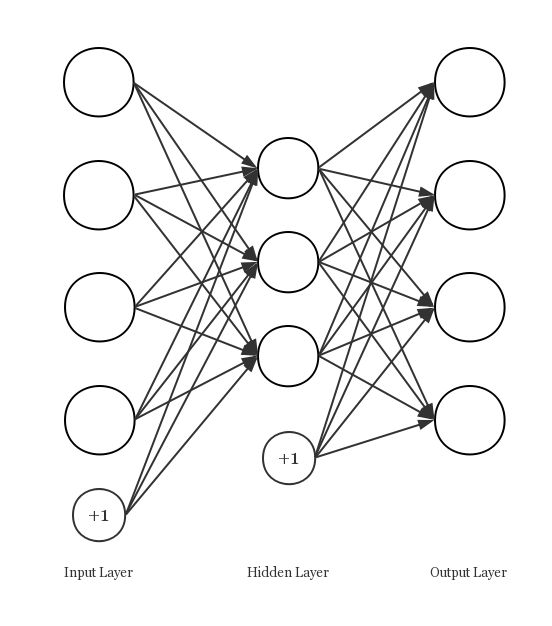
\includegraphics[width=0.45\textwidth]{pictures/autoencoder} %插入图片命令,格式为[配置]{图片路径}
%     }
%     \quad %空格
%     \subfloat[]{
% 	\label{Fig:R2} % 子图2标签名
%     	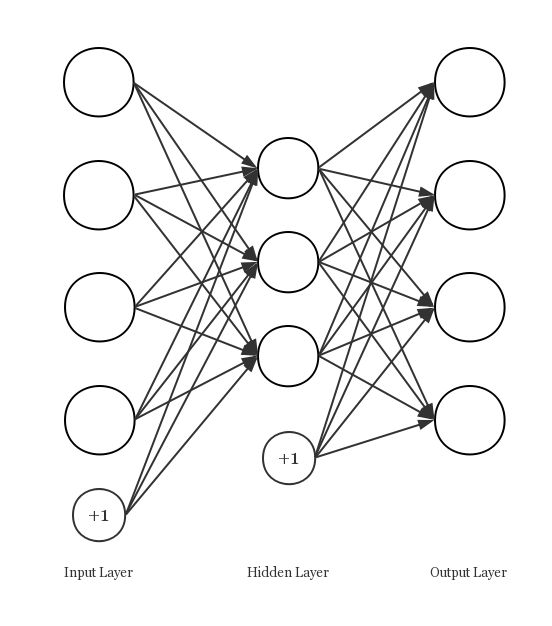
\includegraphics[width=0.45\textwidth]{pictures/autoencoder}
%     }
%     \caption{这是两个自编码器结构,我就是排一下子图的效果:\protect\subref{Fig:R1}左边的自编码器,\protect\subref{Fig:R2}右边的自编码器} %注意须使用\protect\subref{}进行标号引用
%     \label{Fig:RecAccuracy} % 整个组图的标签名
% \end{figure}
%
% \section{公式与算法表示}
%
% \subsection{例子:基于主成分分析}
%
% \subsubsection{主成分分析算法}
%
% 下面对主成分分析进行介绍。
%
% 主成分分析是一种简单的机器学习算法,其功能可以从两方面解释:一方面可以认为它提供了一种压缩数据的方式,另一方面也可以认为它是一种学习数据表示的无监督学习算法。\cite{Goodfellow2016DeepLearning}
% 通过PCA,我们可以得到一个恰当的超平面及一个投影矩阵,通过投影矩阵,样本点将被投影在这一超平面上,且满足最大可分性(投影后样本点的方差最大化),直观上讲,也就是能尽可能分开。
%
% 对中心化后的样本点集$\bm{X}=\{\bm{x}_1,\bm{x}_2,\ldots,\bm{x}_i,\ldots,\bm{x}_m\}$(有$\sum_{i=1}^{m}\bm{x}_i = 0$),考虑将其最大可分地投影到新坐标系\ $\bm{W}= \{\bm{w}_1,\bm{w}_2,\ldots,\bm{w}_i,\ldots,\bm{w}_d\} $,其中$\bm{w}_i$是标准正交基向量,满足$\|\bm{w}_i\|_2 = 1$, $\bm{w}_i^T\bm{w}_j = 0$($i \not= j$)。假设我们需要$d^\prime$($d^\prime < d$)个主成分,那么样本点$\bm{x}_i$在低维坐标系中的投影是$\bm{z}_i = (z_{i1};z_{i2};\ldots;z_{id^\prime})$,其中$z_{ij} = \bm{w}_j^\mathrm{T}\bm{x}_i$,是$\bm{x}_i$在低维坐标系下第$j$维的坐标。
% 对整个样本集,投影后样本点的方差是
% \begin{equation}
% \begin{aligned}
%     & \frac{1}{m}\sum_{i=1}^m \bm{z}_i^\mathrm{T}\bm{z}_i \\
% = & \frac{1}{m}\sum_{i=1}^m (\bm{x}_i^\mathrm{T}\bm{W})^\mathrm{T}(\bm{x}_i^\mathrm{T}\bm{W}) \\
% = & \frac{1}{m}\sum_{i=1}^m \bm{W}^\mathrm{T}\bm{x}_i\bm{x}_i^\mathrm{T}\bm{W} \\
% = & \frac{1}{m} \bm{W}^\mathrm{T}\bm{X}\bm{X}^\mathrm{T}\bm{W} \\
% \end{aligned}
% \end{equation}
%
% 由于我们知道新坐标系$\bm{W}$的列向量是标准正交基向量,且样本点集$\bm{X}$已经过中心化,则PCA的优化目标可以写为
% \begin{equation}
% \label{PCA_goal}
% \begin{aligned}
% & \max_{\substack{\bm{W}}}  &  tr(\bm{W}^\mathrm{T}\bm{X}\bm{X}^ \mathrm{T}\bm{W}) \\
% & \operatorname{ s.t. }  &  \bm{W}^\mathrm{T}\bm{W} = \bm{I} \\
% \end{aligned}
% \end{equation}
%
% 由于$\bm{X}\bm{X}^ \mathrm{ T }$是协方差矩阵,那么只需对它做特征值分解,即
% \begin{equation}
% \label{PCA_eigenvalue}
% \bm{X}^ \mathrm{ T }\bm{X} = \bm{W}\bm{\Lambda}\bm{W}^ \mathrm{ T } \\
% \end{equation}
% 其中$\bm{\Lambda}=diag(\bm{\lambda})$,$\bm{\lambda} = \{\lambda_1,\lambda_2,\ldots,\lambda_m\}$。
%
% 具体地,考虑到它是半正定矩阵的二次型,存在最大值,可对\eqref{PCA_goal}使用拉格朗日乘数法
% \begin{equation}
% \bm{X}\bm{X}^ \mathrm{ T }\bm{w}_i  = \lambda_i \bm{w}_i \\
% \end{equation}
%
% 之后将求得的特征值降序排列,取前$d^\prime$个特征值对应的特征向量组成所需的投影矩阵$\bm{W}^\prime =(\bm{w}_1,\bm{w}_2,\ldots,\bm{w}_{d^\prime})$,即可得到PCA的解。PCA算法的描述如算法\ref{PCA_algorithm}所示。
% \begin{algorithm}
% \floatname{algorithm}{算法}
% \caption{主成分分析(PCA)}
% \label{PCA_algorithm}
% \renewcommand{\algorithmicrequire}{\textbf{输入:}}
% \renewcommand{\algorithmicensure}{\textbf{输出:}}
% \begin{algorithmic}[1]
% \Require 样本集$\bm{x}=\{\bm{x}_1,\bm{x}_2,\ldots,\bm{x}_i,\ldots,\bm{x}_m\}$,低维空间维数$d^\prime$
% \Ensure 投影矩阵  $\bm{W}^\prime =(\bm{w}_1,\bm{w}_2,\ldots,\bm{w}_{d^\prime})$
% \State 对所有样本中心化$\bm{x}_i \gets \bm{x}_i - \frac{1}{m}\sum_{i=1}^m \bm{x}_i$
% \State  计算样本的协方差$\bm{X}\bm{X}^ \mathrm{T}$
% \State 对协方差矩阵$\bm{X}\bm{X}^ \mathrm{T}$做特征值分解
% \State 取最大的$d^\prime$个特征值所对应的特征向量$\bm{w}_1,\bm{w}_2,\ldots,\bm{w}_{d^\prime}$
% \end{algorithmic}
% \end{algorithm}
%
% \subsubsection{主成分分析可信度评估方法}
% 记待判定微博$\bm{w}_0$的经典特征向量为$\bm{f}^{c}_{0}$,它的发布者在$\bm{w_0}$前发布的$k$条微博为$\bm{W} = \bm{w}_1,\bm{w}_2,\ldots,\bm{w}_k$,这$k$条微博对应的经典特征向量集为$\bm{F}^{c}_{W} = \{ \bm{f}^{c}_{1},\bm{f}^{c}_{2},\ldots,\bm{f}^{c}_{k} \}$。令$label = 1$代表谣言,$label = 0$代表非谣言。算法的具体流程如算法\ref{PCA_model}所示。
%
% \begin{algorithm}
% \floatname{algorithm}{算法}
% \caption{基于PCA的信息可信度评估}
% \label{PCA_model}
% \renewcommand{\algorithmicrequire}{\textbf{输入:}}
% \renewcommand{\algorithmicensure}{\textbf{输出:}}
% 	\begin{algorithmic}[1]
% 	\Require $\bm{f}^{c}_{0}$,$\bm{F}^{c}_{W}$,保留主成分数$n$
% 	\Ensure 标签$label\in \{0,1\}$
% 	\State 对所有特征向量应用PCA,保留前$n$个主成分$\bm{o}^{c}_{i} \gets PCA(\bm{f}^{c}_{i}, n)$($i = 0,1,\ldots,k$)
% 	\State 计算$\bm{F}^{c}_{W}$中各向量的平均距离$\mu$和标准差$\sigma$
% 	\State 计算阈值$thr = {\mu} / {\sigma}$
% 	\If {$\min_{1<j\le k} \|\bm{o}^{c}_{0} - \bm{o}^{c}_{j} \|_2 > thr$}
% 		\State $ label \gets 1 $
% 	\Else
% 		\State $ label \gets 0 $
% 	\EndIf
% 	\end{algorithmic}
% \end{algorithm}
%
% \section{代码表示}
% 下面的代码\ref{plus}是用Python编写的加法函数。
%
% \begin{lstlisting}[language=Python, caption=加法, label=plus, tabsize=2]
% def plus_func(a, b):
% 	return a + b
% \end{lstlisting}
%
% \section{列表样式}
%
% 以下是使用圆点作为项目符号的列表样式。
%
% \begin{itemize}
% \item \textbf{第一章为基础模块示例},是的,就是本章。
% \item \textbf{第二章为不存在},是的,其实它不存在。
% \end{itemize}
%
% 以下是使用数字作为项目符号的列表样式。
%
% \begin{enumerate}
% \item \textbf{第一章为基础模块示例},是的,就是本章。
% \item \textbf{第二章为不存在},是的,其实它不存在。
% \end{enumerate}
%
% 以下是无项目符号(实际是可以自定义一些符号,但我懒得加了)的列表样式,它会顶格书写。
%
% \begin{description}
% \item \textbf{第一章为基础模块示例},是的,就是本章。
% \item \textbf{第二章为不存在},是的,其实它不存在。
% \end{description}

%%%%%%%%%%%%%%%%%%%%%%% Main Area ENDs Here %%%%%%%%%%%%%%%%%%%%%%%%
%\let\cleardoublepage=\cleardoublepagebak

% Reference
% \clearpage\phantomsection\addcontentsline{toc}{chapter}{参考文献}
\clearpage\phantomsection\addcontentsline{toc}{chapter}{参考文献}

% \vskip -5cm;
\bibliographystyle{buptbachelor}
\refbodyfont{\bibliography{ref}}

% Thanks to page
\clearpage\phantomsection\addcontentsline{toc}{chapter}{致\qquad{}谢}
\chapter*{致\qquad{}谢}
\normalsize\thankwords

% Appendix
% \setcounter{figure}{0}
% \renewcommand{\thefigure}{~附-\arabic{figure}~}
% \setcounter{equation}{0}
% \renewcommand{\theequation}{~附-\arabic{equation}~}
% \setcounter{table}{0}
% \renewcommand{\thetable}{~附-\arabic{table}~}
%
% \chapter*{附\qquad{}录}
% \phantomsection\addcontentsline{toc}{chapter}{附\qquad{}录}
%
% \phantomsection
% \addcontentsline{toc}{section}{附录1\quad{}缩略语表}
% \section*{附录1\quad{}缩略语表}
%
% \begin{bupttable}{基于浏览者行为的特征}{crowdwisdom}
%     \begin{tabular}{l|l|l}
% 		\hline \textbf{特征} & \textbf{描述} & \textbf{形式与理论范围}\\
% 		\hline 点赞量 & 微博的点赞数量 & 数值,$\mathbb{N}$ \\
% 		\hline 评论量 & 微博的评论数量 & 数值,$\mathbb{N}$ \\
% 		\hline 转发量 & 微博的转发数量 & 数值,$\mathbb{N}$ \\
% 		\hline
%     \end{tabular}
% \end{bupttable}
% \buptfigure[width=0.7\textwidth]{pictures/autoencoder}{自编码器结构}{autoencoder}
%
% \begin{equation}
% \label{PCA_goal}
% \begin{aligned}
% \max_{\substack{\bm{W}}}  &  tr(\bm{W}^\mathrm{T}\bm{X}\bm{X}^ \mathrm{T}\bm{W})
% \end{aligned}
% \end{equation}
%
% \phantomsection
% \addcontentsline{toc}{section}{附录2\quad{}数学符号}
% \section*{附录2\quad{}数学符号}
% \begin{center}
% 	\begin{tabular}{ccc}
% 		\multicolumn{2}{c}{\textbf{数和数组}} \\
% 		\\
% 		$a$ & 标量(整数或实数)\\
% 		$\bm{a}$ & 向量\\
% 		$dim()$ & 向量的维数\\
% 		$\bm{A}$ & 矩阵\\
% 		$\bm{A}^\mathrm{T}$ & 矩阵$\textbf{A}$的转置\\
% 		$\bm{I}$ & 单位矩阵(维度依据上下文而定) \\
%  		$diag(\bm{a})$ & 对角方阵,其中对角元素由向量$\bm{a}$确定 \\
%
% 	\end{tabular}
% \end{center}




%
\newpage\backmatter

% \mbox{}
% \thispagestyle{empty}
% \newpage

% Translated Article
\thispagestyle{empty}
\begin{center}
% 原文第一页,PDF缩放比例为0.95,可以自行调整
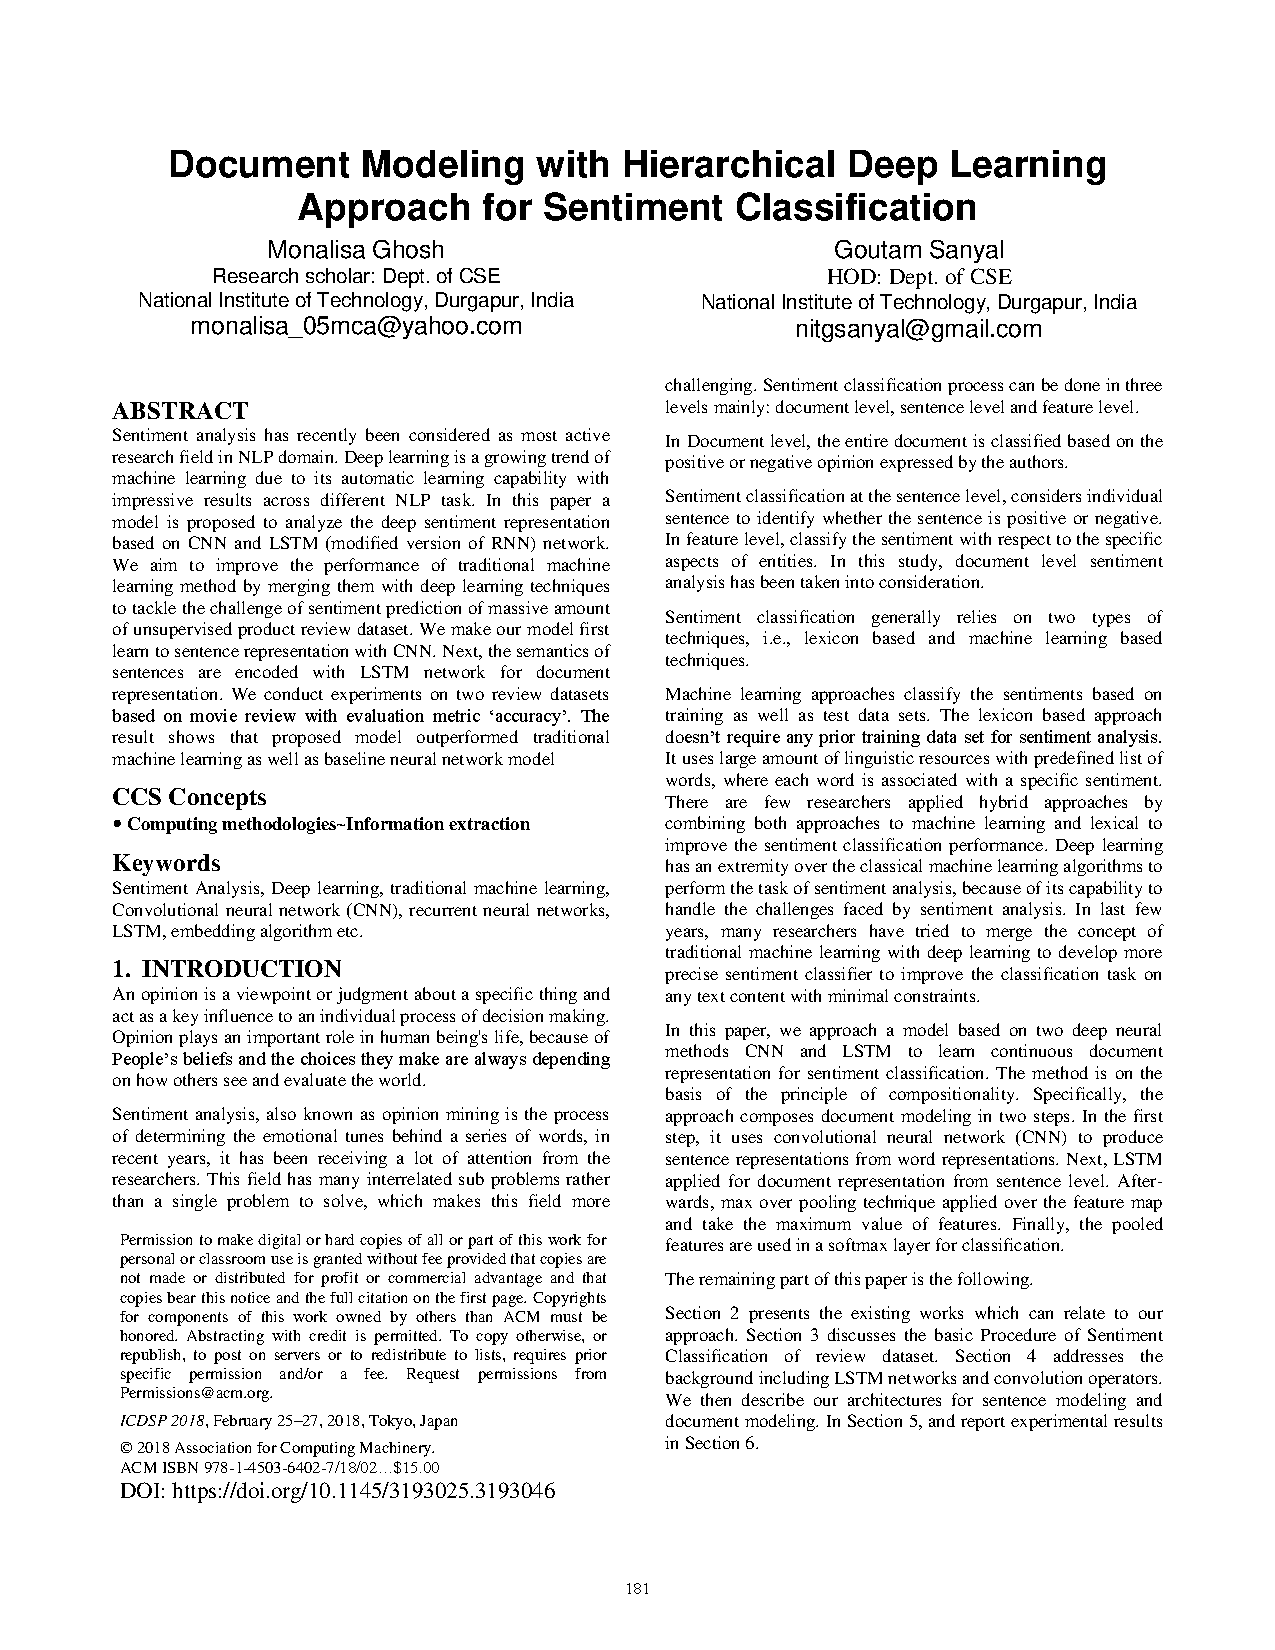
\includepdf[pages=1, scale=0.95, pagecommand=\heiti\sanhao{\textbf{外\quad{}文\quad{}原\quad{}文}}]{docs/translation.pdf}
% 原文剩余部分
\includepdf[pages=2-, scale=0.95, pagecommand={}]{docs/translation.pdf}
\end{center}

\mbox{}
\thispagestyle{empty}
\newpage

% Translation
\chapter*{外\quad{}文\quad{}译\quad{}文}
\vspace{8mm}

\thispagestyle{empty}

\begin{center}
    \sihao\heiti{基于分层深度学习方法的情感分类的文本建模}

\xiaosihao\songti{Monalisa Ghosh, Goutam Sanyal}

\xiaosihao\songti{National Institute of Technology, Durgapur, India}
\end{center}

\songti{}
% \section{摘要}
摘要

情感分析最近在自然语言处理领域,已经被认为是最活跃的研究领域。由于深度学习在多个不同的自然语言处理任务上具有非常可观的成果,因此已经被认为是机器学习的一个热门成长趋势。在这篇文章中,一个基于卷积神经网络(CNN)和长短时记忆(LSTM)网络(循环神经网络(RNN)的修订版本)的模型被推荐来分析深层的情感表达。我们计划期望依靠使用深度学习技巧,来合并这些网络,从而实现处理海量无监督产品评论数据集的情感预测的挑战,从而提高传统机器学习方法的表现能力。首先,我们使用CNN来让我们的模型学习句意表示。其次,使用LSTM网络对句子语义进行编码来实现文本表示。我们在两个电影数据集上进行实现,使用准确度来作为评估单位。结果表示推荐的模型相比传统机器学习模型和基本神经网络模型有所提高。

% \section{关键字}
关键字

情感分析, 深度学习, 传统机器学习, 卷积神经网络(CNN), 循环神经网络, LSTM, 嵌入算法等


% \section{引言}
引言

意见是关于具体事物的观点或判断,对个人决策过程具有十分重要的影响。 意见在人类的生活中发挥着极为重要的作用,因为人们的信仰和选择取决于他人如何看待和评估世界。

情感分析也被称为意见挖掘,是确定一系列词语背后的情感曲调的过程,近年来它一直受到研究人员的大量关注。 这个领域有许多相互关联的子问题,而不是一个要解决的问题,这使得这个领域更具挑战性。 情绪分类过程主要可以分为三个层次:文档层次,句子层次和功能层次。

在文档层面,整个文档根据作者所表达的正面或负面意见进行分类。

在句子级别的情绪分类,考虑单独的句子来确定句子是积极的还是消极的。 在特征层面,将关于实体特定方面的情绪分类。 在这项研究中,文档级的情绪分析已经被考虑在内。

情感分类通常依赖于两种类型的技术,即基于词典的技术和基于机器学习的技术。

机器学习方法基于训练和测试数据集对情绪进行分类。基于词典的方法不需要任何提前训练的数据集来进行情感分析。它使用大量的语言资源和预定义的单词列表,每个单词都与特定的情感有所关联。很少有研究人员将机器学习的方法和基于词典的方法两种方法结合起来应用混合方法来提高情感分析的性能。深度学习相对于用于执行情感分析任务的经典机器学习算法的性能有些优势,因为它能够处理情感分析所面临的挑战。在过去几年中,许多研究人员试图将传统机器学习的概念与深度学习相结合,从而开发更精确的情感分类器,通过最小的约束来改善对任何文本内容的分类任务。

在本文中,我们基于两种深度神经方法卷积神经网络(Convolutional Neural Network,CNN)和长短时程记忆网络(Long Short Time Memory, LSTM)来处理模型,从而学习情感分析的连续文档表示。该方法是基于组合性原则。具体来说,该方法组成文档建模主要分为两步。在第一步中,它使用卷积神经网络(CNN)从单词表示中产生句子表示。接下来,LSTM从句子级别申请文档表示。之后,将max over pooling技术应用于特征映射并获取特征的最大值。最后,汇集的特征用于softmax层进行分类。

本文的其余部分如下。

第2部分介绍了与我们的方法相关的现有工作。第3节讨论审查数据集的情绪分析的基本程序。第4节介绍了包括LSTM网络和卷积算子的知识背景。然后我们描述我们的语句建模和文档建模架构。在第5节中根据实验设计进行实验,并在第6节中根据实验得到的结果进行分析并得到结论。

% \section{相关工作}
相关工作

基于深度学习的神经网络模型在许多NLP相关任务中取得了巨大的成功。 文档级别情感分类是情感分析中的一个基本问题,其目的是识别文档的情感标签。 深度学习的第一个成功的体系结构是基于带有语义向量空间的单词建模[1] [2] [3]。 他们引入了词嵌入技术,每个词都被表示为一个实值向量。 研究人员[4]描述了一个使用动态k-max池操作符的词语模型神经袋。 该模型在没有特征工程的情感分类任务上取得了良好的表现。 Kim [5]将静态向量应用于简单的卷积神经网络,并在不同的数据集上得到了很好的结果。

张等人[6]在2015年提出了用于文本分类的字符级CNN并取得竞争结果。在以前的研究中应用了不同类型的LSTM模型。特别是用两个LSTM [8]分别对假设和假设进行编码的模型,这是一个由Rocktaschel等人应用的共享LSTM [7] .Tai等人提出了树形结构的LSTM。用于情感分类。很少有研究者将CNN和LSTM模型结合起来进行句子分类[9]。 Tang等[10]也应用了CNN和LSTM的层次结构。他们首先使用CNN或LSTM从单词表示中产生句子表示。接下来,应用门控递归神经网络对文档建模语句进行语义编码。

Tai等人(2015)[11]提出将标准LSTM与树形拓扑相结合,并在LSTM的顺序模型上获得了优越的结果。在[12]中,研究人员提出了三种不同的模型,用于循环神经网络的多任务学习。

Vo等人[13]为情绪引入了一个越南语料库分类,这是从越南商业网站收集的页面。他们申请CNN和LSTM来生成信息越南情绪分析渠道。魏等人。接近[14]基于卷积神经网络和长期短期记忆模型的转移学习框架。该体系结构自动识别帖子是否表达混乱,确定帖子的紧迫性并最终将极性分类。

% \section{基本理论}
基本理论

在我们的工作中,我们遵循基于机器学习方法进行情感分类的基本过程。分类方法总结为几个步骤,如下所述。

A.审查数据集进行预处理,以便可以应用监督学习算法。数据处理需要通过考虑标记化,停用词删除,词干方法来消除噪音,不一致和不完整。

B.本建议考虑的功能是基于POS的固定模式中的Unigram功能和双字(双标记)功能。通过结合unigram和bitagged功能创建的复合功能集。

C.用于为每个单独特征和最高排序特征分配特定分数的Tf-Idf方法将被视为监督ML算法的输入。

D.最后,训练具有不同特征向量的监督机器学习分类器SVM和NB以对数据集进行分类。 SVM和NB分类器被认为是评估我们提出的模型的基准方法。

% \buptfigure[width=0.7\textwidth]{pictures/translation_1}{使用机器学习方法进行情感分类的基本框架的体系结构}{translation_1}

% \section{推荐模型}
推荐模型

长期短期记忆(LSTM)网络在以前关于情感分类问题的研究中表现出色。 这是通过处理这个问题来模拟远距离依赖的递归神经网络的修改版本。 这种深度学习网络的关键要素是记忆单元,信息可以记忆在其中。 在我们的方法中,为了对文档语义表示进行建模,我们采用长短期记忆(LSTM)网络和卷积神经网络(CNN),通过结合词级和句级的分层结构。

卷积神经网络由一个或多个卷积层和顶端的全连通层(对应经典的神经网络)组成,同时也包括关联权重和池化层(pooling layer)。这一结构使得卷积神经网络能够利用输入数据的二维结构。与其他深度学习结构相比,卷积神经网络在图像和语音识别方面能够给出更好的结果。这一模型也可以使用反向传播算法进行训练。相比较其他深度、前馈神经网络,卷积神经网络需要考量的参数更少,使之成为一种颇具吸引力的深度学习结构。

卷积层是构建卷积神经网络的核心层,它产生了网络中大部分的计算量。卷积层的参数是有一些可学习的滤波器集合构成的。每个滤波器在空间上(宽度和高度)都比较小,但是深度和输入数据一致。举例来说,卷积神经网络第一层的一个典型的滤波器的尺寸可以是5x5x3(宽高都是5像素,深度是3是因为图像应为颜色通道,所以有3的深度)。在前向传播的时候,让每个滤波器都在输入数据的宽度和高度上滑动(更精确地说是卷积),然后计算整个滤波器和输入数据任一处的内积。当滤波器沿着输入数据的宽度和高度滑过后,会生成一个2维的激活图(activation map),激活图给出了在每个空间位置处滤波器的反应。

LSTM通过输入门、遗忘门、输出门结构来控制循环神经网络中的各个时刻的状态。这里所说的三种门实际上是sigmoid神经网络和一个按位做乘法的操作,形象的来说,sigmoid激活函数的全连接神经网络会输出0到1之间的数值,表示这个结构保留下来的信息。

我们考虑有多个卷积滤波器的CNN从每个不同大小的窗口捕捉局部特征[10],其中每个滤波器被视为特征检测器。 由于卷积层的输出长度基于输入句子的长度,因此我们的方法中使用最大共享层来保持句子向量大小的一致性。 与简单平均相比,该层用于分类任务的性能更好。 我们更喜欢CNN和LSTM是文档级和句子级分类的最新组合模型[5] [4] [15]。 在我们的方法中,我们不需要任何外部解析器或解析结果来捕获高质量句子表示的长距离依赖关系。 近年来,基于CNN的模型[23]在各种NLP任务中表现出色,例如用于类别预测[4] [5],对象识别[17]和其他传统NLP任务[16]的句子和文档建模等。

我们来讨论一下LSTM和CNN网络如何使用它来学习文档语义表示。 首先我们定义词向量表示。 作为预训练的通用词向量可以通过词嵌入学习算法(word2vec)来提取[2] [1]。 有时词汇向量以无监督的方式捕捉到语义和句法信息。 在我们的方法中,我们考虑未经训练的词向量。 一般来说,我们假设产品p∈P包含来自用户的评论。 该评论可以表示为具有N个句子{s1,s2,...,.sN}的文档d。然后考虑,句子J-th的长度是1J。 第J个句子由j个词组成,如J J J {w 1,w 2,...,w l J},CNN的卷积滤波器用于从句子sJ中提取局部特征。

% \subsection{词语等级}
词语等级

每个单词表示为连续的和实值的矢量,我们将这个单词嵌入到一个低维空间中[21]。 这个过程被称为词嵌入[18]。 以这种方式,每个词w i映射到其嵌入表示J w iεR d和滤波器FεR d×| L | ,这里d是单词向量的维数,L是窗口的大小。
LSTM网络可以产生隐藏状态表示[19]。 对于句子sJ的给定单词𝑤1,单元格的当前状态和隐藏状态分别为𝑐𝑡和ℎ𝑡可以用𝐽𝐽前一个单元状态𝑐1 -1和隐藏ℎ𝑡-1更新为 时间步t按以下方式。
% \buptfigure[width=0.7\textwidth]{pictures/translation_formula_1}{}{translation_formula_1}
其中σ表示逻辑斯蒂尔德函数,ʘ表示单元乘法。 请注意,(i,f,o)是使用忘记门ft,输入门和输出门ot激活门。 这些门决定如何将单元从一个状态更新到另一个状态。 W {i,f,o,c},b {i,f,o,c}是我们必须训练的一组参数。
% \subsection{句子模型}
句子模型


% \buptfigure[width=0.7\textwidth]{pictures/translation_2}{句子模型样例}{translation_2}

根据CNN由多层共享参数组成。 每个图层执行将其输入交替为有用表示的特定任务。 我们尝试使用CNN作为第二层来组成句子模型。 这个卷积神经网络由多个不同宽度的卷积滤波器组成。 在这项工作中,我们应用三个不同宽度的卷积滤波器来获取Ngrams的本地语义,例如句子中的unigrams,bigrams和trigrams。 假设一个句子作为n个词[w 1,w 2,w 3 ...,w k,... w n]的输入。 让我们考虑p和b是共享参数,l是滤波器F的窗口大小。对于CNN层w iεR d是维数为d的单词w i的嵌入表示。 通常,线性层的输入是字嵌入的连接,如w i:i + l-1 = {w i,w i + 1,... .w i + l-1}εR dl。 现在我们可以如下确定线性层的输出O= p. w+b

其中,pε𝑅𝑙𝑜×和bε𝑅𝑙𝑜×是共享参数,l o被认为是线性层的输出长度。 接下来,为了提取句子的全局特征,我们将线性图层的输出提供给最大时间池图层。 在卷积神经网络的顶部添加最大随时间汇聚层。 最后,汇集的特征用于softmax层进行分类。
% \subsection{文本模型}
文本模型

% \buptfigure[width=0.7\textwidth]{pictures/translation_3}{文本模型样例}{translation_3}

我们提出的体系结构不限于句子建模,所提供的句子向量被提供来组成文档模型。 让我们考虑处理后的文档作为我们模型的输入,其中文档由n个句子[s 1,s 2,s 3,...,s n]组成。 我们将LSTM应用于文档组合,其方式与语句建模相同。 LSTM网络的隐藏状态反馈给平均共享层。 这样,我们得到了句子的平均值。
CNN将被置于LSTM的顶部,如句子建模。 最后,分类任务可以通过最大池和softmax层的泳池特征来完成。

% \section{实验}
实验

% \subsection{数据集}
数据集

在本节中,我们进行实验来评估我们模型在各种基准数据集上的有效性。 我们的主要任务是对这些不同的域数据集进行情感分类。 具体来说,我们使用电影评论和电影评论数据集来评估我们模型的性能,并与现有的基线模型进行比较。 这两个数据集的评估指标是准确度。 除非另有说明,我们认为80%的数据用于培训目的,10%用于验证,其余10%用于测试。
SST2:Stanford Sentiment Treebank是电影评论数据集的延伸。 它与SST1相同,但该评论数据集仅包含二进制标签。

IMDB电影评论数据集包含5,331个正面评论和5,331个负面评论,电影评论[22]
% \subsection{预处理}
预处理

标记或分段:可以通过将文档分成单词列表来完成。 在我们的实验中,我们使用Stanford Tokenizer来获取令牌。

停用词的去除:某些高频停用词将被删除(介词,无关词)。
% \subsection{实验设置}
实验设置


我们基于Python库实现我们的模型。 深度学习神经网络的超参数设置可能取决于用于实验的数据集。 对于产品评论数据集,我们考虑了超参数,例如滤波器数量,CNN中的滤波器长度; 记忆维度在LSTM; 要应用哪一层等等。在我们提出的架构中,我们使用一个CNN层和一个LSTM层。 滤波器大小或滤波器长度1,2,3用于单个卷积层捕获局部特征。

% \subsection{对照方法}
对照方法


我们将我们提出的模型与以下基准方法进行比较,包括传统的机器学习方法,如SVM,NB等,用于文档级别情感分类。
% \subsubsection{传统范式}
传统范式

\begin{itemize}
    \item SVM + Ngrams:基于SVM的方法与Unigram,Bigram和Unigram + Bigram一样精心制作[10]。
    \item NB + Ngrams:具有Unigram特征和Bigram特征的朴素贝叶斯分类器[4]也被认为是基线方法。
    \item NBSVM-bi:[20]以前的研究指定了SVM和具有两个特征的多项式NB。
    \item 文本特征是基于[24]定义的,其中包括单词和字符ngrams,情感词汇特征,群集特征等。
\end{itemize}
% \subsubsection{神经网络范式}
神经网络范式

\begin{itemize}
    \item CNN-rand,CNN-static,CNN-nonstatic和CNNmultichannel:文[5]提出的CNN模型的这四种变体基于用于情感分类的词向量的不同用法。

    \item 标准LSTM:标准长期短期记忆网络[11]被认为是比较我们的方法的基线。
\end{itemize}
% \section{结果讨论}

结果讨论

我们提出的模型在不同数据集上的实验结果如表1所示。这个结果集中了与其他基线方法相比的有效性。 我们使用度量“精度”评估每个数据集,每个数据集中最好的方法将用粗体标出。

% \buptfigure[width=0.7\textwidth]{pictures/translation_4}{}{translation_4}

\textbf{表1.与电影评论数据集上的基准模型的比较。 二进制是一个2分类任务。 第一个块包含传统方法的其他基线方法。 与卷积神经网络有关的第二种阻塞方法。 第三个块包含用于字表示和Char表示的CNN方法。 第四个块包含使用LSTM的方法。 最后一块是我们的模型。}

从表1可以看出,对于不同的数据集,神经网络方法(CNN,LSTM)优于传统方法。 神经网络方法在组成文本数据的语义表示方面更有效。 但是,必须指出,SVM分类器与Ngram特征相比是非常强大的方法,与其他基准方法相比较。

当使用电影评论数据集将卷积神经网络和递归神经网络(RNN)与递归NN进行比较时,基于CNN的方法实现更好的准确性。 这是因为RNN患有梯度消失和梯度爆炸问题。 长期短期记忆模型(LSTM)等改进版本的RNN在句子和文档建模方面的效果非常好。

% \section{结论}
结论

在本文中,我们引入神经网络模型(Neural Network)进行文档级情感分类。 该方法是首先用长短期记忆网络学习句子表示,然后用卷积神经网络对文本表示语义进行编码。 我们基于评估度量“准确度”的电影评论对两个评论数据集进行实验。 结果表明,该模型比传统的机器学习和基准神经网络模型在情感分类数据集上具有更高的准确率。





% 开题报告
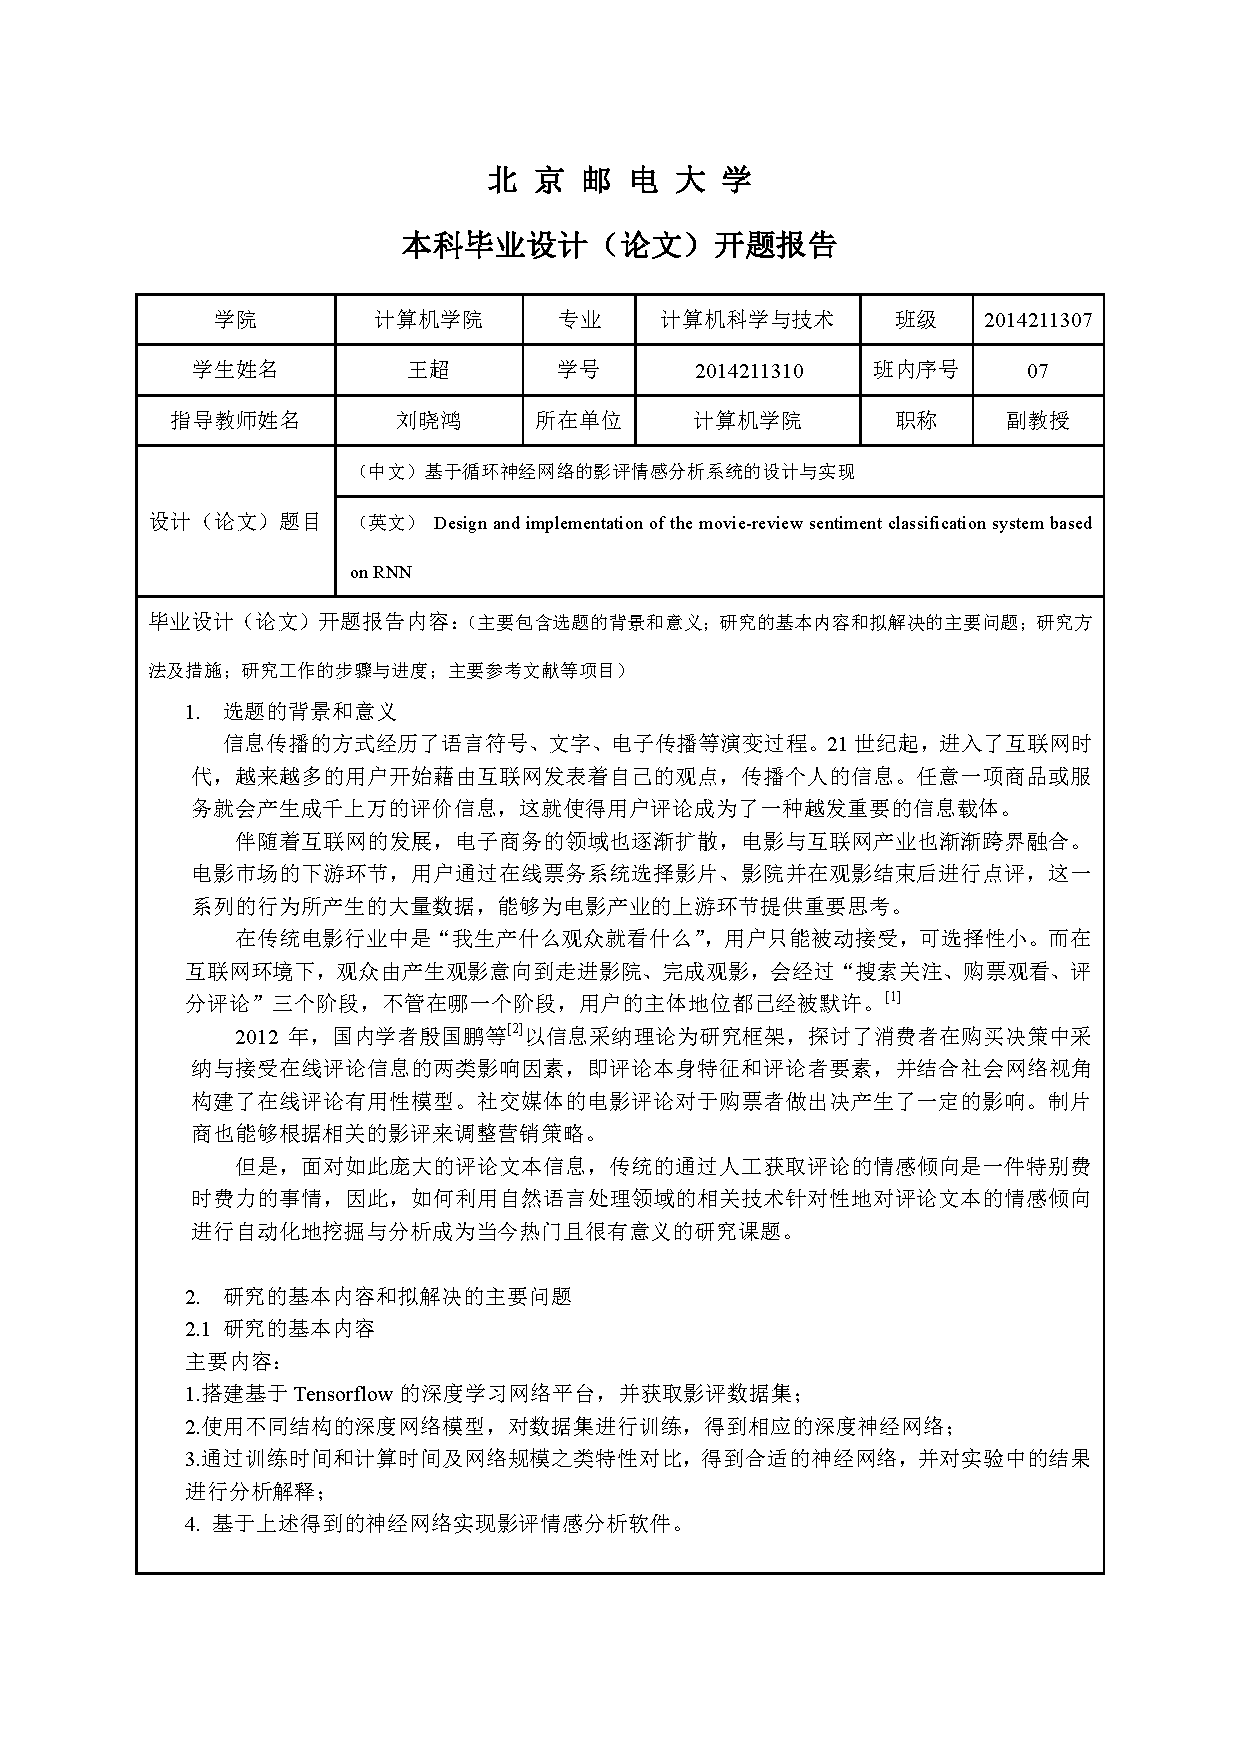
\includepdf[pages=-]{docs/openingReport.pdf}

\mbox{}
\thispagestyle{empty}
\newpage

% 中期检查表
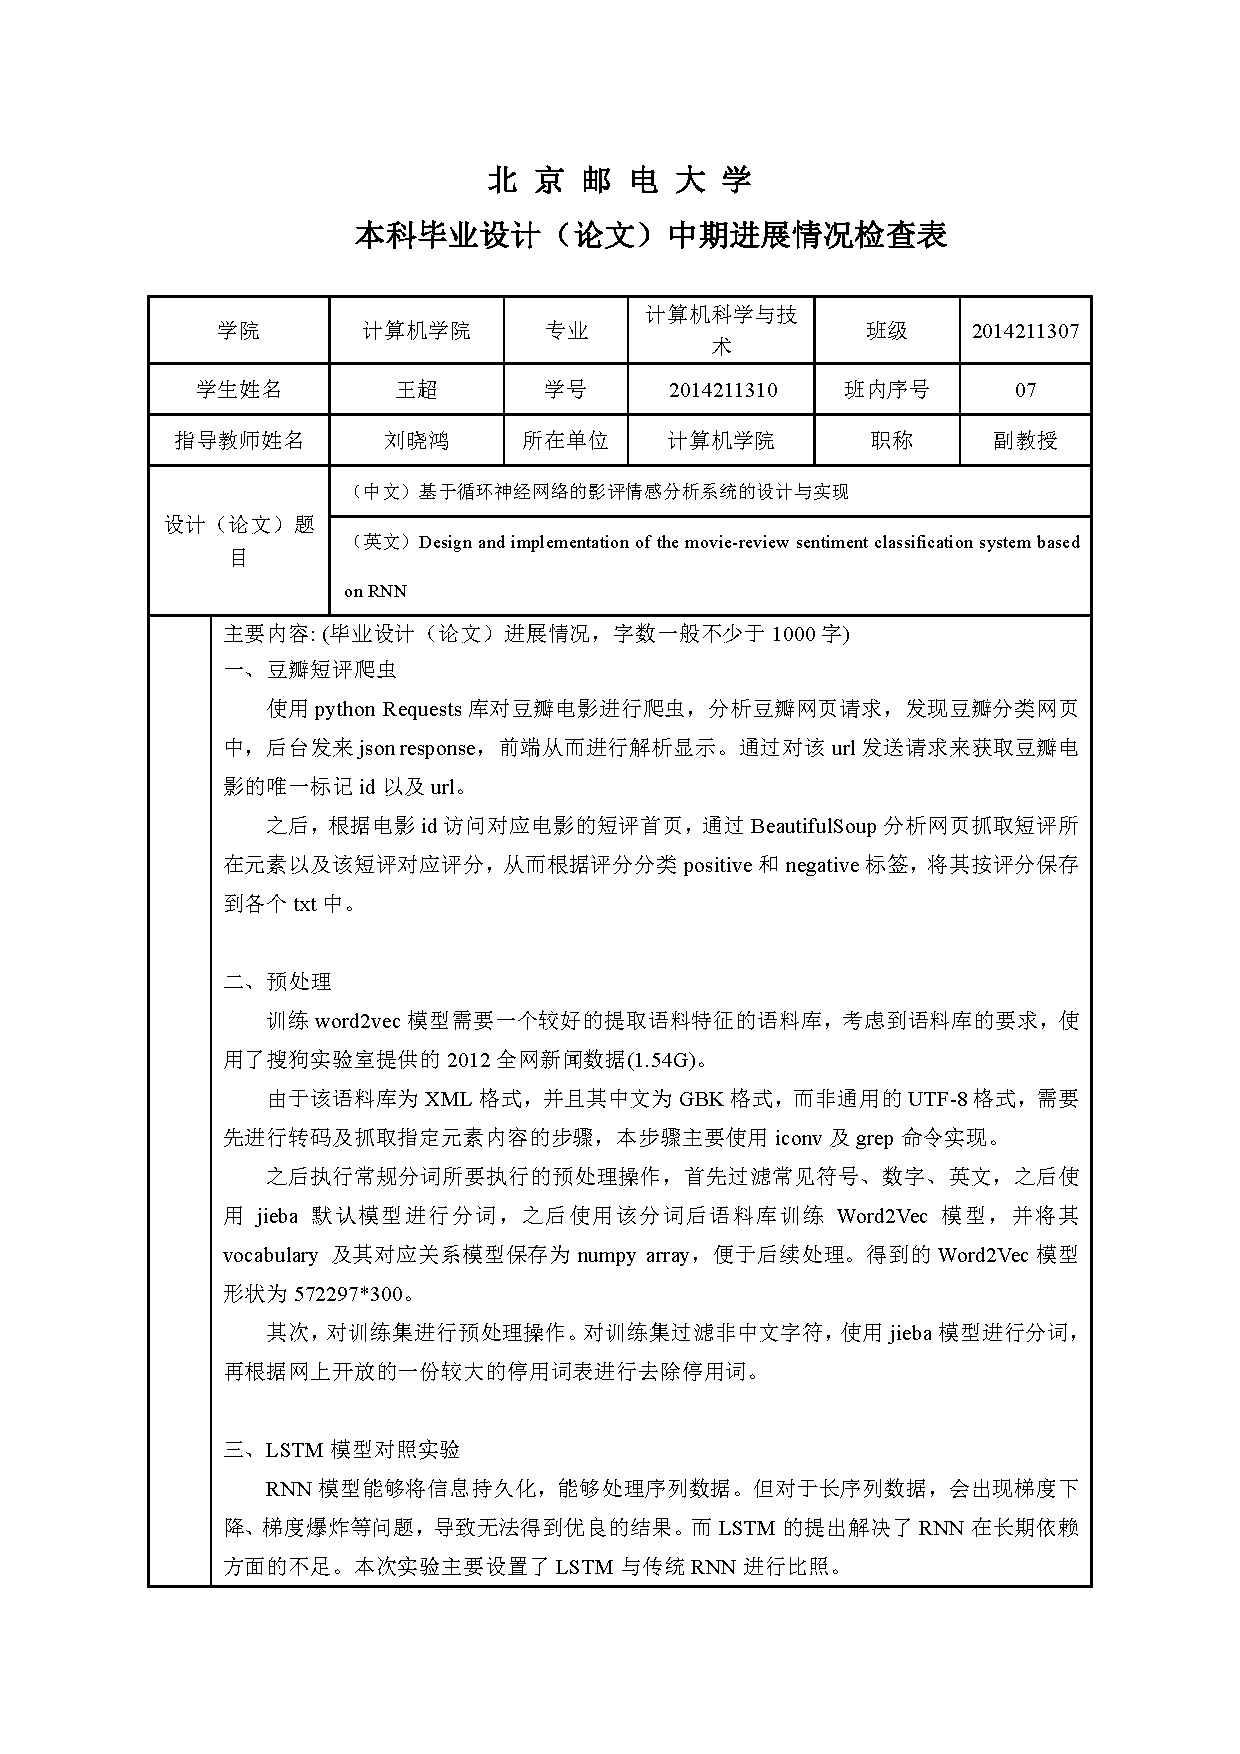
\includepdf[pages=-]{docs/interimReport.pdf}


\end{document}
